\documentclass{article}
\usepackage[left=2.5cm,right=2.5cm, top = 2.5cm, bottom = 3cm]{geometry}
\usepackage{graphicx}
\usepackage{natbib}
\usepackage{hyperref}
\usepackage{todonotes}
\usepackage{booktabs}
\usepackage{amssymb}
\usepackage{amsmath}

\newcommand{\sd}{s}
\newcommand{\mean}{\bar{y}}


\begin{document}
% \SweaveOpts{concordance=TRUE}

% \title{A bootstrap-based comparison of ILI intensity thresholds from the moving epidemic and WHO methods}
\title{A statistical assessment of influenza intensity thresholds from the moving epidemic and WHO methods}
\author{Johannes Bracher$^{1, 2}$, Jonas M. Littek$^1$}
\date{9 June 2023\\ \medskip \small
$^1$Karlsruhe Institute of Technology (KIT), Chair of Statistics and Econometrics\\
$^2$Heidelberg Institute for Theoretical Studies (HITS), Computational Statistics Group}

\maketitle

\begin{center}
\textbf{This manuscript is is a preprint and has not been subject to peer review.}
\end{center}


\abstract{
\begin{quote}
\footnotesize Intensity thresholds serve to make influenza activity comparable across countries and surveillance systems. The moving epidemic method (MEM) and the WHO method are widely used to classify season peaks as low, medium, high or very high. In both methods, thresholds correspond to quantiles of a normal distribution fitted to a set of potentially transformed historical observations. However, there are differences in how this set is constructed. We assess the impact of these choices analytically and in simulation studies. We find that under the default settings of both the MEM and WHO method, on average more season peaks than intended are classified as high or very high. Combining characteristics of both, better-calibrated thresholds can be achieved. Even these, however, must be expected to have rather modest positive predictive values and should be interpreted with care.
\end{quote}
}

\begin{center}
\textbf{Author's summary}
\end{center}

{\begin{quote}
\footnotesize Intensity thresholds are a common tool to make influenza activity comparable across different countries and surveillance systems. The moving epidemic method (MEM) and the WHO method are widely used to this end and enable classification of season peak intensity as low, medium, high or very high. The two approaches are similar in that they base thresholds on quantiles of a normal distribution fitted to a reference set of historical observations. However, three methodological differences exist. Firstly, in the MEM the normal distribution is fitted to log-transformed incidence data, while the WHO method by default operates on the original scale. Secondly, the MEM uses more than one observation from each past season, fixing the total number to include into the reference set. The WHO method uses only the highest value from each season. Lastly, in the WHO method, but not the MEM, historical data are by default  smoothed prior to the computation of thresholds. We assess the impact of these choices on thresholds both analytically and in a simulation study. The latter is based on re-sampling of influenza-like illness (ILI) data from France and the US, thus reflecting temperate climate settings. We find that when the normal distribution is fitted to untransformed observations, a rather large proportion of new season peaks are classified as high or very high intensity. This can be mitigated by a logarithmic transformation. When fixing the total number of past observations included in the reference set as in the MEM, thresholds increase in expectation the more seasons are available. When only few are available, there is a high chance of classifying new season peaks as high or very high intensity. Smoothing incidence time series prior to computing thresholds results in somewhat less variable estimators, but also a lowering of thresholds. If these are applied to unsmoothed new season peaks, there will again be a large proportion classified as high or very high intensity. If they are applied to smoothed new data, this problem is avoided. In terms of sensitivity and positive predictive values of thresholds, we find that these cannot be expected to exceed rather modest levels if the number of available historical seasons is low; thresholds for very high intensity are particularly affected by this problem. Our practical recommendation is to include one observation per season into the reference set and employ a log transformation in the computation of thresholds. Smoothing can be applied to somewhat reduce the variability of thresholds. However, threholds then need to be applied to smoothed rather than raw new peak values, which slightly modifies their interpretation.
\end{quote}}

\bigskip

\begin{quote}
\textbf{Keywords:} calibration, influenza, intensity threshold, moving epidemic method, re-sampling, sensitivity, WHO method.
\end{quote}

\newpage

%\textbf{Points Moss and H\"ohle:}
%\begin{itemize}
%\item Remove past outliers?
%\item Type of distribution (normal) is problematic
%\item cumulative or peak?
%\item need to add smoothing aspect:
%\begin{itemize}
%\item 3-week in Rguig
%\item 4 weeks in WHO guideline and one other (re-check)
%\end{itemize}
%\end{itemize}
%
%New points:
%\begin{itemize}
%\item discuss general difficulty of estimating extreme values from few observations
%\item mention that it is worse for extreme quantiles
%\item do we classify the "right" seasons as extreme? FPR?
%\item trends / discarding?
%\end{itemize}


% \medskip

% \noindent \textbf{Keywords:} influenza-like illness, intensity thresholds, moving epidemic method, seasonal influenza, WHO method

\section{Introduction}

Influenza intensity thresholds are a common tool to make influenza activity comparable across different countries and surveillance systems. Based on data from past influenza seasons, they provide a classification into \textit{low}, \textit{medium}, \textit{high} or \textit{very high} intensity. While thresholds are designed to assess the season peak intensity, they are also used to monitor spatial and temporal patterns over the course of a season. To this end, intensity classifications are commonly summarized in heat charts and maps; see Figure \ref{fig:maps} for an example from the \textit{Flu News Europe} platform run by the World Health Organization (WHO) and the European Center for Disease Prevention and Control (ECDC). Intensity thresholds thus play an important role in assessing the influenza situation at an international level.

\begin{figure}[h!]
\begin{center}
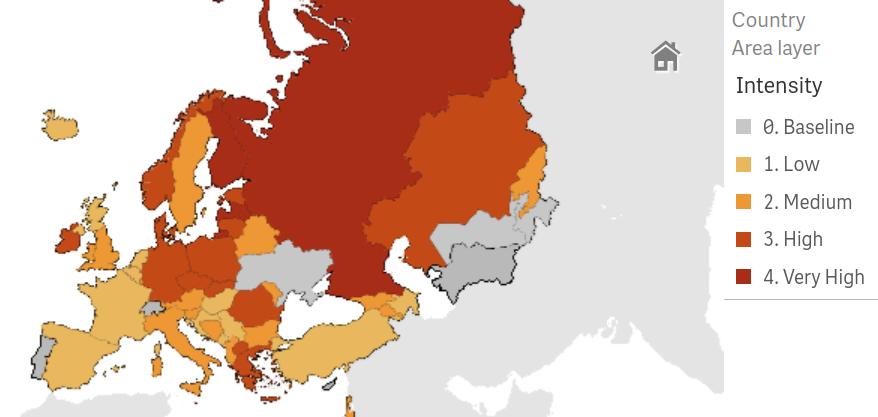
\includegraphics[width=0.6\textwidth]{figure/maps.png}

\medskip

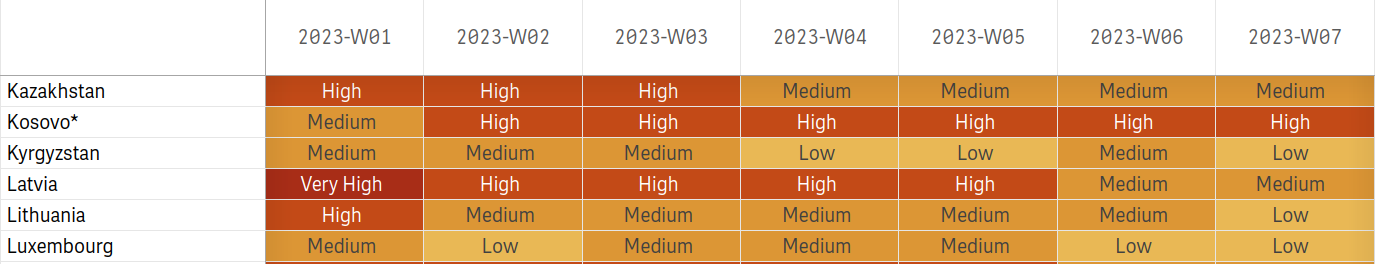
\includegraphics[width=0.8\textwidth]{figure/heat_chart.png}
\end{center}
\caption{Influenza intensity map (top, week 01/2023) and heat chart (bottom, weeks 01--07/2023) as published by \textit{Flu News Europe} (\url{https://flunewseurope.org/SeasonOverview}). Copyright: World Health Organization 2023 and European Centre for Disease Prevention and Control 2023.
Reproduction is authorised, provided the source is acknowledged}
\label{fig:maps}
\end{figure}

Following the 2009 influenza H1N1 pandemic, the \textit{Review Committee on the Functioning of the International Health Regulations and on Pandemic Influenza (H1N1)} recommended that member states apply and evaluate their methods for severity assessment every year, thus improving their pandemic preparedness \citep[p.118]{WHO2011}. In the subsequent \textit{WHO Pandemic Infuenza Severity Assessment (PISA)} guideline \citep{WHO2017}, two statistical methods were recommended to determine influenza intensity thresholds. These are the so-called \textit{WHO method} \citep{WHO2014} and the \textit{moving epidemic method} (MEM; \citealt{Vega2015}) which has also been recommended by the European Centre for Disease Prevention and Control (e.g., \citealt{ECDC2017}). As will be detailed in Section \ref{sec:definitions}, the WHO and MEM approaches bear important similarities and can be seen as variations of the same general approach.

Especially the moving epidemic method has been adopted by many national public health agencies, and a large number of articles documenting practical applications exist (see Section \ref{sec:review}). The theoretical statistical properties of the MEM and WHO methods, however, have not yet been studied in detail. In the present work, we aim to close this gap and derive some recommendations for the computation of influena intensity thresholds. We obtain some analytical results, complemented by simulation experiments based on re-sampling of real-world data from France and the US. These indicate that using the recommended default settings, both the moving epidemic and the WHO methods tend to produce too low thresholds, leading to a higher number of season peaks classified as high or very high intensity than intended. The best behaviour of thresholds is achieved by combining characteristics of the MEM and WHO methods. Even the recommended configuration, however, is characterized by rather modest sensitivity and positive predictive values unless data on many historical seasons are available. This concerns in particular the threshold for very high intensity and should be kept in mind when using both the MEM and WHO method.

The remainder of the article is structured as follows. Section \ref{sec:desirable_properties} lists several desirable properties of a threshold setting procedure. Section \ref{sec:definitions} provides definitions of the MEM and WHO methods, highlighting three differences between these otherwise similar approaches. Section \ref{sec:review} consists of an overview of published applications of the MEM and WHO methods. This is followed by an examination of statistical properties of the two methods in Section \ref{sec:analytical_results}. In Section \ref{sec:simulation} we conduct the simulation study before concluding with a discussion in Section \ref{sec:discussion}. Here we also provide practical recommendations on the different implementation choices.


\section{Desirable properties of a thresholding method}
\label{sec:desirable_properties}

We start by stating properties of a thresholding method for influenza activity which we consider desirable. These will guide the analyses in the remainder of the paper.

\begin{description}
\item \textbf{Calibration.} As stated in the \textit{WHO Pandemic Influenza Severity Assessment} guideline, the rationale for both the MEM and the WHO method is that
\begin{quote}
\textit{``about 50--60\% of the season peaks should be above the moderate threshold, $\pm 10\%$ above the high threshold and $\pm 2.5\%$ above the extraordinary threshold''} \citep[p.10]{WHO2017}.
\end{quote}
This is a purely statistical definition, and threshold setting corresponds to estimating quantiles of an underlying distribution of season peak values. A major requirement for the thresholds is thus \textit{calibration}. We call a method calibrated if in the long run, the right fractions of seasons are classified as low, medium, high and very high. If, for instance, a method flags new season peaks as very high intensity in considerably more than 2.5\% of the cases, this will hamper the usefulness of thresholds.
\item \textbf{Sensitivity and specificity.} In addition to classifying the right number of seasons into the various categories, the individual classifications should be correct. A season peak exceeding the very high/high/medium threshold should indeed be among the 2.5\%/10\%/60\% most extreme season peaks according to the underlying true distribution. Conversely, a season peak which is not actually among the 2.5\%/10\%/60\% most extreme ones should not be flagged as such. As a complementary perspective to sensitivity and specificity, confusion matrices can be considered to assess how peaks which are truly very high, high, medium or low intensity are classified. % The true distribution of season peaks is of course unknown in practice, but the sensitivity and specificity of a given method can be studied theoretically and in simulation studies.
\item \textbf{Stability.} Estimated thresholds should not be overly variable. Ideally they would not fluctuate strongly around the corresponding quantiles of the true distribution of season peaks.
\item \textbf{Simplicity.} To ensure broad practical applicability, understanding the thresholding method should not require advanced statistical training. The method should be simple enough that a quantitatively literate user can develop a good intuition of its functioning and parameters.
\item \textbf{Ease of practical application.} Besides conceptual simplicity, ease of application is central. Methods should be straightforward to apply using well-documented and ideally open-source software packages.
\end{description}

\noindent We note that while the overarching goal of the \textit{WHO PISA} guidelines is to enhance preparedness for \textit{pandemic influenza}, the intended statistical properties of the MEM and WHO methods refer to \textit{seasonal influenza waves}. The rationale is that a good understanding of the range of peak intensities of seasonal influenza is the basis for a meaningful assessment of pandemic influenza outbreaks. Our reasoning in the following therefore focuses on this setting of subsequent waves of seasonal influenza. Note that we only address the question of peak intensity thresholds, but not season onset / baseline thresholds \citep{Vega2013}. Also, we do not address the question of determining peak intensity in real time, i.e., before the season peak has been reached or before it is clear whether a peak has been reached. Rather than simple thresholds, this would require control charts (see e.g., \citealt{Liu2019}), which we consider outside the scope of the present article.

\section{Definition of the moving epidemic and WHO methods}
\label{sec:definitions}

While framed slightly differently in the respective documentations, the MEM and WHO methods can be seen as two special cases of the same general approach. We assume that thresholds are based on weekly data (typically incidences) from $m$ past seasons and applied to the ($m + 1$)-th season. Implicitly it is further assumed that each influenza season consists of just one wave and does not feature multiple peaks separated by longer time spans. This is typically the case in temperate, but not necessarily in tropical regions. Thresholds are are then obtained as follows.

\begin{enumerate}
\item \textbf{Smoothing of historical data} (optional): apply an $l$-week moving average to all historical seasons. If data are smoothed, we denote by $x^\text{raw}_{j, k}$ the raw observation from season $j = 1, \dots, m$, week $k = 1, \dots, 52$, and by
$$
x^\text{smo}_{j, k} = \frac{1}{l} \sum_{d = 0}^{l - 1} x^\text{raw}_{j, k - d}, \ \ k = l, \dots, 52
$$ the smoothed version. In the remainder of this description we denote whichever of $x^\text{raw}_{j, k}$ and $x^\text{smo}_{j, k}$ is used to compute thresholds by $x_{j, k}$.
\item \textbf{Sorting:} Within each historical season $j = 1, \dots, m$ order all observations $x_{j, k}$ in decreasing order, denoting the $i$-th largest observation from season $j$ by $x^{(i)}_j$.
\item \textbf{Selection of reference set:} Select the $n$ largest observations from each of the $m$ past seasons to construct a reference set $\mathcal{X} = \{x_j^{(i)}: j = 1, \dots, m; i = 1, \dots, n\}$.
\item \textbf{Data transformation:} Apply a monotonically increasing transformation $y_j^{(i)} = f(x_j^{(i)})$ to all members of the reference set $\mathcal{X}$ to obtain a reference set $\mathcal{Y}$ of transformed historical observations.
\item \textbf{Fitting a normal distribution:} Assume that the transformed values in $\mathcal{Y}$ come from a normal distribution and compute estimates of its mean and standard deviation,
\begin{align}
\begin{split}
\bar{y} & = \frac{\sum_{j = 1}^m\sum_{i = 1}^n y_j^{(i)}}{nm}\\
\sd & = \sqrt{ \frac{\sum_{j = 1}^m\sum_{i = 1}^n (y_j^{(i)}  - \bar{y})}{nm - 1}}.
\end{split}\label{eq:moments}
\end{align}
\item \textbf{Computation of thresholds:} Define intensity thresholds on the transformed scale as quantiles of the normal distribution N$(\bar{y}, \sd^2)$, i.e.\ compute
\begin{equation}
\hat{q}_{Y, \alpha} = \bar{y} + z_\alpha \sd, \label{eq:def_q}
\end{equation}
where $z_\alpha$ is the $\alpha$ quantile of the standard normal distribution. These can be interpreted as estimates of quantiles $q_{Y, \alpha}$ of an underlying theoretical distribution. A common choice is
\begin{itemize}
\item the 40th percentile $\hat{q}_{Y, 0.4} = \bar{y} - 0.25 \sd$ as the threshold for medium intensity;
\item the 90th percentile $\hat{q}_{Y, 0.9} = \bar{y} + 1.28 \sd$ as the threshold for high intensity;
\item the 97.5th percentile $\hat{q}_{Y, 0.975} = \bar{y} + 1.96\sd$ as the threshold for very high intensity.
\end{itemize}
\item \textbf{Transformation of thresholds to original scale:} Obtain corresponding thresholds on the original scale by applying the inverse transformation, i.e. setting % $\hat{q}_{X, 0.4} = f^{-1}(\hat{q}_{Y, 0.4})$, $\hat{q}_{X, 0.9} = f^{-1}(\hat{q}_{Y, 0.9})$, $\hat{q}_{X, 0.975} = f^{-1}(\hat{q}_{Y, 0.975})$.
$$
\hat{q}_{X, \alpha} = f^{-1}(\hat{q}_{Y, \alpha})
$$
for $\alpha = 0.4, 0.9, 0.975$.
\item \textbf{Application of thresholds:} The obtained thresholds are applied to classify the season peak value of the next season. Depending on the exact specification, thresholds can be applied either to the raw peak value $x_{m + 1}^{\text{raw}, (1)}$ or the smoothed version $x_{m + 1}^{\text{smo}, (1)}$.
\end{enumerate}

\noindent The MEM and WHO methods are special cases of this procedure, see also overview in Table \ref{tab:differences}. In the MEM method, no smoothing is applied and the default data transformation $f$ is the natural logarithm.  \cite{Vega2015} recommend to use $5 \leq m \leq 10$ seasons to ensure a recent data basis. The number of observations included per season is set to $n = 30/m$, rounded to the nearest integer (with a minimum value of $n = 1$). The total number of historical observations is thus kept approximately fixed. We note that this description refers to the specification from \cite{Vega2015}, which is also reflected in the default settings of the accompanying R package \texttt{mem} \citep{Lozano2020}. The package, however, permits the user to choose $n$, $m$, and $f$ (\texttt{i.type.intensity	= 5} for no transformation, \texttt{i.type.intensity = 6} for the log transformation), thus offering considerable flexibility. We note that while \texttt{mem} does not currently allow for data smoothing using a moving average, alternatives like LOESS (locally estimated scatterplot smoothing) are available. % The term \textit{moving epidemic method} could thus also be used as an umbrella term for the general procedure described above. We here use it in a more narrow sense for the specification from \cite{Vega2015}, reflected in the default settings of the \texttt{mem} package.
% \begin{itemize}
% \item

The implementation of the WHO method in the publicly available \textit{WHO Average Curves} application \citep{WHO2023} likewise offers a lot of flexibility; our description is based on the default settings as of May 2023, as well as the description in \cite{WHO2014}. Smoothing of data prior to the computation of thresholds is recommended, with a default of $l = 3$ (adapted from a recommendation of $l = 4$ in \citealt[p68]{WHO2014}). Subsequently, $n = 1$ observation per season is used and by default no transformation is applied to the reference set. If peak incidences vary strongly across seasons, a log transformation is recommended. At least three historical seasons are required to compute thresholds, but it is noted that the ``accuracy of these thresholds should be expected to increase with the number of seasons of good quality data available'' \cite[p22]{WHO2023}. % \citep{WHO2017}.
Thresholds are by default applied to unsmoothed new season peaks.

Both the inclusion of multiple observations per season in the MEM ($n > 1$) and the smoothing of data in the WHO method ($l > 1$) can be seen as attempts to base estimation of thresholds on more data than just one peak value per historical season. This is intended to make estimation more stable. The impact of these strategies on the resulting thresholds will be discussed in Section \ref{sec:analytical_results}.


% \item

% \end{itemize}

\begin{table}[h]
\caption{Default settings of the moving epidemic and WHO methods.}
\label{tab:differences}
\begin{center}
\footnotesize
\begin{tabular}{lll}
\toprule
& moving epidemic method & WHO Method \\
\midrule
smoothing of historical data & none & moving average, $l = 3$\\
number $n$ of observations used per season & $n = \max[\text{round}(30/m), 1]$ & $n = 1$\\
default transformation for reference set & natural logarithm & none\\
recommended number $m$ of historical seasons & $5 \leq m \leq 10$ & $m \geq 3$, more recommended\\
smoothing of new season peak & none & none\\
\bottomrule
\end{tabular}
\end{center}

\end{table}



% \noindent In the following we will study analytically and empirically how these different analytical choices impact the resulting thresholds.

% \subsection{Hypothesized properties}

\section{Review of recent use cases}
\label{sec:review}

To improve our understanding of the different settings in which the MEM and WHO methods are applied in practice we performed a literature search of articles published in English language and citing the papers \cite{Vega2015}, \cite{WHO2014} and \cite{WHO2017} until December 2020 (identified via \textit{CrossRef} and \textit{Google Scholar}). The results are summarized in Table \ref{tab:literature}. As can be seen from the large number of entries from the years 2019 and 2020, the MEM has quickly become a standard approach in the determination of intensity thresholds for influenza and other respiratory diseases. The articles come from numerous countries and in many cases have been co-authored by representatives of national or regional public health agencies. In most analyses, threshold levels at the 40th, 90th and 97.5th percentile as in Section \ref{sec:definitions} are used. Variability with respect to the number $m$ of historical seasons included is considerable, with a range from 3 to 16 seasons. Consequently, the number $n$ of observations included per season ranges from two to ten (none of the above papers indicated a modification of the default setting $n = 30/m$ of the moving epidemic method). We only found three published applications of the WHO method, one of them providing a comparison to the thresholds from the MEM method \citep{Rguig2020}.

\begin{table}[h!]
\caption{Applications of the MEM and WHO method to determine intensity thresholds for respiratory diseases. We did not include works where only baseline thresholds are computed. The number of seasons included to compute thresholds is denoted by $m$, the number of observations used per season by $n$. The ``Percentiles'' column indicates which percentiles were used for the medium, high and very high thresholds, with ``?'' indicating that no explicit information was found. Abbreviations: SARI = severe acute respiratory infection; ILI = influenza-like illness; RSV = respiratory syncytial virus.}
\label{tab:literature}
\center
\footnotesize
\begin{tabular}{l l l l l l l}
\multicolumn{7}{c}{(a) Moving epidemic method}\\ \\

\toprule
Region & Disease & Years covered & $m$ & $n$ & Percentiles & Authors\\
\midrule
Australia & ILI/influenza & 2012--2017 & 5 & 6 & 40, 90, 99 & \cite{Vette2018}\\
Australia, Chile, & ILI/SARI & 2013--2019 & 6 & 5 & 40, 90, 97.5 & \cite{Sullivan2019}\\
New Zealand,\\
South Africa\\
Catalonia & ILI & 2010--2016 & 5 & 6 & ? & \cite{Basile2018}\\
Catalonia & ILI & 2005--2018 & 12 & 3 & ? & \cite{Basile2019}\\
Catalonia & ILI/influenza & 2010--2017 & 7 & 4 & ? & \cite{Torner2019}\\
Egypt & SARI/ILI & 2010--2017 & 6 & 5 & 40, 90, 97.5 & \cite{AbdElGawad2020}\\
Egypt & SARI & 2013--2015 & 3 & 10 & ? & \cite{Elhakim2019}\\
England & ILI & 2010--2016 & 6 & 5 & ? & \cite{Wagner2018}\\
Finland & influenza & 2011--2016 & 5 & 6 & ? & \cite{Pesaelae2019}\\
Montenegro & ILI & 2010--2018 & 7 & 4 & 40, 90, 97.5 & \cite{Rakocevic2019}\\
Morocco & ILI & 2005--2017 & 11 & 3 & 40, 90, 97.5 & \cite{Rguig2020}\\
Netherlands & RSV & 2005--2017 & 12 & 3 & 40, 90, 97.5 & \cite{Vos2019}\\
Norway & influenza & 2006--2015 & 9 & 3 & ? & \cite{Benedetti2019}\\
Pakistan & ILI, SARI & 2008--2017 & 10 & 3 & 40, 90, 97.5 & \cite{Nisar2020}\\
Portugal & ILI & 2012--2017 & 5 & 6 & 40, 90, 97.5 & \cite{Pascoa2018}\\
Scotland & influenza & 2010--2018 & 7 & 4 & ? & \cite{Murray2018}\\
Scotland & influenza & 2010--2019 & 7--8 & 4 & 40, 90, 97.5 & \cite{Dickson2020}\\
Slovenia & RSV & 2008--2018 & 10 & 3 & 40, 90, 97.5 & \cite{Grilc2021}\\
Spain (17 regions) & ILI & 2003--2015 & 4--10 & 3--8 & 40, 90, 97.5 & \cite{Bangert2017}\\
Spain & ILI & 2001--2018 & 16 & 2 & 40, 90, 97.5 & \cite{RedondoBravo2020}\\
Tunisia & ILI & 2009-2018 & 9 & 3 & 50, 90, 95 & \cite{Bouguerra2020}\\
United Kingdom & ILI & 2000--2013 & 10 & 3 & 40, 90, 97.5 & \cite{Green2015}\\
United Kingdom & ILI/RSV & 2011--2018 & 4--6 & 5--8 & 40, 90, 97.5 & \cite{Harcourt2019}\\
USA & ILI/influenza & 2003--2015 & 11 & 3 & 50, 90, 98 & \cite{Biggerstaff2017}\\
USA & ILI & 2010--2015 & 5 & 6 & 50, 90, 98 & \cite{Dahlgren2018}\\
USA & influenza & 2010--2016 & 6 & 5 & 50, 90, 98 & \cite{Dahlgren2019}\\
\bottomrule\\
\multicolumn{7}{c}{(b) WHO method}\\ \\
\toprule
Region & Disease & years covered & $m$ & $n$ & percentiles & authors\\
\midrule
Cambodia & ILI & 2009--2015 & 7 & 1 & mean, 90, 95 & \cite{Ly2017}\\
Morocco & ILI & 2005--2017 & 11 & 1 & 40, 90, 97.5 & \cite{Rguig2020}\\
Philippines & ILI & 2006--2012 & 7 & 1 & 90 & \cite{Lucero2016}\\
Victoria/Australia & ILI & 2002--2011 & 6--10 & 1 & 90, 95 & \cite{Tay2013}\\
\bottomrule\\
\end{tabular}
\end{table}



\section{Analytical results on statistical properties}
\label{sec:analytical_results}

Both the MEM and WHO method essentially serve to estimate quantiles of the distribution of season peak values ($q_{X, 0.4}, q_{X, 0.9}, q_{X, 0.975}$) from historical data. In the following we obtain some analytical results on how the estimators ($\hat{q}_{X, 0.4}, \hat{q}_{X, 0.9}, \hat{q}_{X, 0.975}$) behave under different variations of the procedure outlined in Section \ref{sec:definitions}. In all cases we will simplifyingly assume that the available historical seasons are independent realizations of the same random process, i.e., we ignore time trends, correlations between neighbouring seasons and other changes in seasonal patterns. To highlight that we treat all incidence values as random rather than observed variables in this section, we will denote them by capital rather than lowecase letters (e.g., $X_j^{(i)}$ rather than $x_j^{(i)}$). All derivations are provided in Supplement \ref{appendix:derivations}.


\subsection{Choice of number $n$ of observations used per season}
\label{subsec:choice_n}

We first consider the impact of the number $n$ of observations used per historical season. We assume that no smoothing is applied in Step 1 of the algorithm described in Section \ref{sec:definitions}. Denote by $\mathbf{Y}_j$ the random vector of the $n$ largest transformed incidence values from season $j$ in decreasing order, i.e.
$$
\mathbf{Y}_j = (Y^{(1)}_j, \dots, Y^{(n)}_j)^\top.
$$
We assume that $\mathbf{Y}_1, \dots, \mathbf{Y}_m$ are identically and independently distributed, denoting their theoretical mean and covariance matrix of by
\begin{align}
\mathbb{E}\left(\mathbf{Y}_j\right) = \boldsymbol{\mu} = \left(\begin{array}{c}
\mu_1\\
\vdots\\
\mu_n
\end{array}\right) \ \ \ \text{and} \ \ \ \text{Cov}\left(\mathbf{Y}_j\right) = \boldsymbol{\Sigma} =
\left(\begin{array}{ccc}
\sigma_{1, 1} & \cdots & \sigma_{1, n}\\
\vdots & \ddots &\vdots\\
\sigma_{n, 1} & \cdots & \sigma_{n, n}
\end{array}\right).
\end{align}
To make notation more intuitive we also write $\sigma^2_i = \sigma_{i, i}$. Construction of thresholds is based on the reference set $\mathcal{Y}$, which pools the elements of the vectors $\mathbf{Y}_1, \dots, \mathbf{Y}_m$. It can be shown that the expectations of $\bar{Y}$ and $S^2$ as defined in equation \eqref{eq:moments} are given by
\begin{align}
\mathbb{E}(\bar{Y}) & = \frac{1}{n} \sum_{i = 1}^n \mu_i,
\label{eq:expectation_mu}\\
\mathbb{E}(S^2) & = \frac{m}{mn - 1} \sum_{i = 1}^n (\sigma_{i}^2 + \mu_i^2) \ - \ \frac{1}{n(mn - 1)} \sum_{i = 1}^n \sum_{i' = 1}^n \sigma_{i,i'} \ - \ \frac{m}{n(mn - 1)}\left(\sum_{i = 1}^n \mu_i\right)^2,
\label{eq:expectation_sigma2}
\end{align}
%\begin{align}
%\mathbb{E}(\mean) & = \frac{1}{K} \sum_{i = 1}^K \mu_i,
%\label{eq:expectation_mu}\\
%\mathbb{E}(\sd^2) & = \frac{n}{nK - 1} \sum_{i = 1}^K (\sigma_{i}^2 + \mu_i^2) \ - \ \frac{1}{K(nK - 1)} \sum_{i = 1}^K \sum_{i' = 1}^K \sigma_{i,i'} \ - \ \frac{n}{K(nK - 1)}\left(\sum_{i = 1}^K \mu_i\right)^2,
%\label{eq:expectation_sigma2}
%\end{align}
respectively. Moving to the resulting thresholds,
\begin{align}
\mathbb{E}(\hat{q}_{Y, \alpha}) & \approx \mathbb{E}(\bar{Y}) + z_\alpha \sqrt{\mathbb{E}(S^2)}
\label{eq:expectation_q}\\
\mathbb{E}(\hat{q}_{X, \alpha}) & \approx f^{-1}\left\{\mathbb{E}(\bar{Y}) + z_\alpha \sqrt{\mathbb{E}(S^2)}\right\}
\label{eq:expectation_q2}
\end{align}
usually holds in good approximation in our applied setting if the transformation function $f$ is the identity or the natural logarithm; see Appendix \ref{appendix:derivation_n} for details. It can further be shown that for $n = 1$ the approximation becomes
$$
\mathbb{E}(\hat{q}_{Y, \alpha}) \approx \mu_1 + z_\alpha \sigma_1 = q_{Y, \alpha},
$$
where the second equality holds only if the transformed peak values $Y_{j}^{(1)}$ indeed come from a normal distribution.  This is a desirable property as our estimator of the relevant quantile is approximately unbiased. In expectation, thresholds on the transformed scale are thus such that the nominal threshold exceedance probabilities (60\%/10\%/2.5\%) are achieved. If a different value $n > 1$ is chosen, this will generally no longer be the case. Equations \eqref{eq:expectation_mu}--\eqref{eq:expectation_q} tell us by how much $\hat{q}_{Y, \alpha}$ can then be expected to differ from $q_{Y, \alpha}$. By the definition of $\mu_i$ as the expectation of the $i$-th largest observation in a given season, $\mathbb{E}(\bar{Y})$ decreases in $n$. While the expected thresholds also depend on $\mathbf{\Sigma}$, this downward bias will usually translate to the $\hat{q}_{Y, \alpha}$. As a consequence, when choosing $n > 1$, one must expect to classify a larger number of season peaks as high or very high intensity. Intuitively speaking, extending the reference by observations which are close to peaks, but not actually peaks, dilutes the reference set and pulls thresholds downward. When choosing $n = 30/m$ as suggested for the MEM, thresholds will tend to increase the more years of data are used to compute thresholds, and the probability of exceeding thresholds will decrease (approaching the nominal values from above). 

% Intuitively speaking, if $n = 1$ one observation per season is used, the reference set contains only actual peak values. The set may thus be small, but only contains observations which -- being season peaks themselves -- provide a good reference for future peaks. If $n > 1$, the set becomes larger, but at the cost of a systematic downward bias resulting from the inclusion of non-peak weeks.



\subsection{Smoothing of time series prior to computing of thresholds}
\label{subsec:smoothing}

Next we assess the role of smoothing historical data prior to computing thresholds. As derivations get tedious otherwise, we only consider the case where $f$ is the identity function, i.e., no transformation is applied to the reference set and thus $
Y^{(i)}_j = X^{(i)}_j$. Also, as smoothing and multiple observations per season are generally not used in parallel we assume $n = 1$.

Now denote by $p_j$ the peak week of the smoothed incidence in season $j$ such that $X_j^{(1)} = X^{\text{smo}}_{j, p_j}$; and by
$$
\mathbf{X}^\text{raw}_j = (X_j^{\text{raw}, (1)}, \dots, X_j^{\text{raw}, (l)})^\top
$$
the random vector containing the raw observations $X^\text{raw}_{j, p_j - l + 1}, X^\text{raw}_{j, p_j - l + 2}, \dots, X^\text{raw}_{j, p_j}$ in decreasing order. The vector $\mathbf{X}^\text{raw}_j$ is thus a re-ordering of the raw observations making up the smoothed peak value. The theoretical mean and covariance matrix of $\mathbf{X}^\text{raw}_j$ are denoted by
\begin{align}
\mathbb{E}\left(\mathbf{X}^\text{raw}_j\right) = \boldsymbol{\mu}^\text{raw} = \left(\begin{array}{c}
\mu^\text{raw}_1\\
\vdots\\
\mu^\text{raw}_n
\end{array}\right) \ \ \ \text{and} \ \ \ \text{Cov}\left(\mathbf{X}^\text{raw}_j\right) = \boldsymbol{\Sigma}^\text{raw} =
\left(\begin{array}{ccc}
\sigma^\text{raw}_{1, 1} & \cdots & \sigma^\text{raw}_{1, n}\\
\vdots & \ddots &\vdots\\
\sigma^\text{raw}_{n, 1} & \cdots & \sigma^\text{raw}_{n, n}
\end{array}\right),
\end{align}
respectively. Note that by construction we have $\mu^\text{raw}_1 \geq \mu^\text{raw}_2 \geq \dots > \mu^\text{raw}_l$. As we assumed $f$ to be the identity and $n = 1$, the reference set $\mathcal{Y}$ consists simply of $Y^{(1)}_1, \dots, Y^{(1)}_m$ with
$$
Y^{(1)}_j = X^{\text{smo}}_{j, p_j} = \frac{1}{l} \sum_{d = 1}^l X^{\text{raw}, (i)}_{j},
$$
i.e., the average values of $\mathbf{X}^\text{raw}_{1}, \dots, \mathbf{X}^\text{raw}_{m}$. It is straightforward to show that in this case the expectations of $\bar{Y}$ and $S^2$ are
\begin{align}
\mathbb{E}(\bar{Y}) = \frac{1}{l} \sum_{i = 1}^l \mu^\text{raw}_i, \ \ \ 
\mathbb{E}(S^2) = \frac{1}{l^2} \sum_{i = 1}^l \sum_{i' = 1}^l \sigma^\text{raw}_{i', i}.
\label{eq:expectation_moments_smoothing}
\end{align}
These can be plugged into equation \eqref{eq:expectation_q} to approximate the expected thresholds. Similarly to the previous section, for $l = 1$ we obtain
\begin{equation}
\mathbb{E}(\hat{q}_{Y, \alpha}) \approx \mathbb{E}(\bar{Y}) + z_\alpha \sqrt{\mathbb{E}(S^2)} \approx \mu^\text{raw}_1 + z_\alpha \sigma^\text{raw}_1.
\label{eq:expected_threshold_smooth}
\end{equation}
Now assume that the peak of the raw time series is always part of the vector $\mathbf{X}_j^\text{raw}$ and thus has mean $\mu^\text{raw}_1$ and standard deviation $\sigma^{2, \text{raw}}_1$. This will typically be the case if a season presents one well-shaped peak. If in addition the normality assumption holds, then equation \eqref{eq:expected_threshold_smooth} implies that the threshold $\hat{q}_\alpha$ is again approximately unbiased. % in the sense that in expectation they are such that the unsmoothed peak of a new season will exceed them with the intended probabilities (60\%/10\%/2.5\%).
For $l > 1$ we get by construction $\mathbb{E}(\bar{Y}) \leq \mu^\text{raw}_1$ and usually also $\mathbb{E}(\sqrt{S^2}) \leq \sigma^\text{raw}_1$. In practice both are likely to hold in strict inequality. The high and very high thresholds will thus be lower than for $l = 1$ and exceeded more frequently by unsmoothed new peaks. If thresholds are applied to new smoothed peak values, though, the nominal exceedance probabilities will be achieved in expectation as the mean and variance of the smoothed peak values correspond to the expressions from equation \eqref{eq:expectation_moments_smoothing}.

As in Section \ref{subsec:choice_n}, the key aspect is that the reference set need to be comparable to new peaks; both smoothed peak values and values which are close to, but not actually peaks are systematically different from new unsmoothed peak values. They are thus not suitable as reference values, and the resulting thresholds will be biased. While we did not adapt our derivation to the case where data are log-transformed prior to computing thresholds, our simulation results in Section \ref{subsec:sim_smoothing} confirm that the described qualitative patterns likewise hold.



\subsection{Sensitivity and specificity under normality and $n = 1$}
\label{subsec:theory_sensitivity}

While in the previous sections we focused on the expected thresholds, we now turn to the resulting sensitivity and specificity. An implicit assumption of the MEM and WHO methods is that the observations in the reference set $\mathcal{Y}$ as well as the new transformed season peak $Y_{m + 1}^{(1)}$ are identically and independently normally distributed; as discussed in Section \ref{subsec:choice_n}, this assumption is implausible if $n > 1$, so we focus on the case where $n = 1$ observation is used per historical season and thus $\mathcal{Y} = \{Y_1^{(1)}, Y_2^{(1)}, \dots, Y_m^{(1)}\}$. The normality assumption is then
$$
Y_1^{(1)}, \dots, Y_m^{(1)}, Y_{m + 1}^{(1)} \stackrel{\text{i.i.d.}}{\sim} \text{N}(\mu_1, \sigma^2_1).
$$
Defining the threshold $\hat{q}_{Y, \alpha}$ via equations \eqref{eq:moments} and \eqref{eq:def_q}, it can be shown that
\begin{equation}
\hat{q}_{Y, \alpha} \stackrel{\text{approx}}{\sim} \text{N}\left[\mu_1 + z_\alpha \sigma_1,\ \ \sigma_1^2 \times \left(\frac{1}{m} + \frac{z_\alpha^2}{2(m - 1)} \right) \right].
\label{eq:q_Y}
\end{equation}
Based on this we can compute the sensitivity and specificity of our thresholding procedure at level $\alpha$. The sensitivity describes the probability that given
$$
Y_{m + 1}^{(1)} \geq q_{Y, \alpha} = \mu_1 + z_\alpha \sigma_1,
$$
i.e., the new transformed peak is in theory among the $(1 - \alpha) \times 100\%$ highest peaks, it will also be classified as such, i.e.,
$$
Y_{m + 1}^{(1)} \geq \hat{q}_{Y, \alpha}.
$$
Note that we here treat both $Y_{m + 1}^{(1)}$ and $\hat{q}_{Y, \alpha}$ as random. It can be shown that the probability in question can be approximated by
\begin{equation}
\text{sens}_\alpha = \text{Pr}(Y_{m + 1}^{(1)} > \hat{q}_{Y, \alpha} \ \mid \ Y_{m + 1}^{(1)} > q_{Y, \alpha}) \approx \int_{z_\alpha}^\infty \phi(x) \times \Phi\left(\frac{x - z_\alpha}{\sqrt{\frac{1}{m} + \frac{z_\alpha^2}{2(m - 1)}}}\right) \text{d}x,
\label{eq:sens}
\end{equation}
where $\phi$ and $\Phi$ are the standard normal density function and cumulative density function, respectively. We note that this expression only depends on $\alpha$, but not $\mu_1$ and $\sigma^2_1$. Similarly, the specificity can be approximated by
\begin{equation}
\text{spec}_\alpha = \text{Pr}(Y_{m + 1}^{(1)} < \hat{q}_\alpha \ \mid \ Y_{m + 1}^{(1)} < q_{Y, \alpha}) \approx \int_{-\infty}^{z_\alpha}\phi(x) \times \left[1 - \Phi\left(\frac{x - z_\alpha}{\sqrt{\frac{1}{m} + \frac{z_\alpha^2}{2(m - 1)}}}\right)\right] \text{d}x.
\label{eq:spec}
\end{equation}
The positive predictive value can be computed using the common formula
\begin{equation}
\text{PPV}_\alpha = \text{Pr}(Y_{m + 1}^{(1)} > q_{Y, \alpha} \ \mid Y_{m + 1}^{(1)} > \hat{q}_\alpha) = \frac{(1 - \alpha) \times \text{sens}_\alpha}{(1 - \alpha) \times \text{sens}_\alpha + \alpha \times (1 - \text{spec}_\alpha)}.
\label{eq:ppv}
\end{equation}
Neither of these expressions has any simpler closed form, but they are straightforward to evaluate numerically. We visualize the resulting curves in Figure \ref{fig:sens_spec_ana}. As the approximations are derived under the assumption of large $m$ while in our setting $m$ is typically small, we also show simulation-based versions. The simulations indicate that the theoretical sensitivity for small $m$ is slightly higher than in the approximation, but otherwise agreement is quite close. Little surprisingly, the sensitivity, specificity and positive predictive values increase in $m$. The sensitivity and PPV are lowest for the very high threshold at $\alpha = 0.975$. For the most practically relevant values of $5 \leq m \leq 10$, the PPV is only between 0.25 and 0.4 in this case. More than half of the seasons flagged as very high intensity will thus be false positives. For the high threshold ($\alpha = 0.9$), the respective PPVs are between 0.5 and 0.6. Even if the underlying normality assumptions are fulfilled, there are thus natural limits to the classification performance, which for small $m$ and high $\alpha$ is at relatively modest levels. We note that this general theoretical result is the same irrespective of
 whether smoothing has been applied to all peaks in question or not. While smoothing will usually make thresholds less variable, any effect on sensitivity and specificity is canceled out by the fact that smoothed new peaks are likewise less variable.

\begin{figure}
\begin{center}
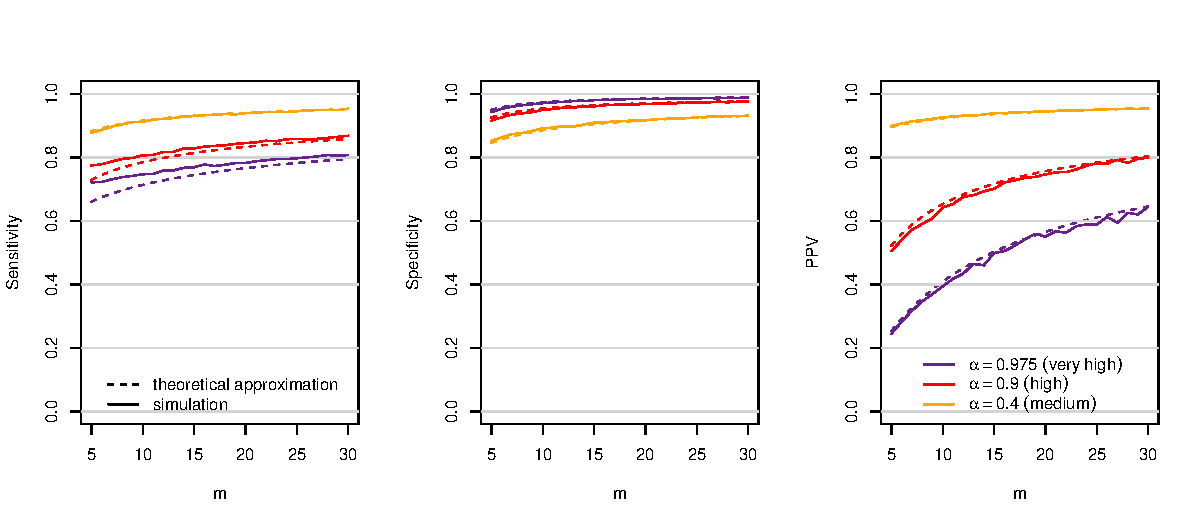
\includegraphics[scale=0.75]{figure/analytical_sens_spec.pdf}
\end{center}

\vspace{-10mm}

\caption{Sensitivity, specificity and positive predictive values under normality assumption, by number $m$ of historical seasons used. Solid lines show a theoretical approximation, dashed lines simulation results.}
\label{fig:sens_spec_ana}
\end{figure}



\subsection{Basing thresholds on confidence intervals}
\label{subsec:cis}

In previous works (\citealt{WHO2014, Vega2015}), the thresholds as defined in Section \ref{sec:definitions} have been described as upper ends of one-sided confidence intervals for the arithmetic (WHO method) or geometric mean (MEM) of the reference observations. This, however, is imprecise terminology as in the computations the standard deviation $\sd$ rather than the standard error $\sd/\sqrt{nm}$ is used (see documentation of the \texttt{mem} package and \citealt{WHO2014}, p.69). The intervals thus correspond to prediction rather than confidence intervals. The use of actual confidence intervals is also possible in the \texttt{mem} package (\texttt{i.type.intensity = 1} for the geometric, \texttt{i.type.intensity = 2} for the arithmetic mean). Under this specification, equation \eqref{eq:expectation_q} becomes
$$
\mathbb{E}(q_{Y, \alpha}) \approx \mathbb{E}(\bar{Y}) + \frac{z_\alpha}{\sqrt{nm}} \sqrt{\mathbb{E}(S^2)}.
$$
This is not a desirable property as given enough historical observations (large $mn$), thresholds for all levels $\alpha$ will converge to $\mathbb{E}(\bar{Y})$. Each new season will then be classified either as low or as very high.

\section{Simulation study}
\label{sec:simulation}

\subsection{Simulation setup}
\label{subsec:simulation_setup}

The analytical results from Section \ref{sec:analytical_results} involve some simplifying approximations and the assumption that the observations in the reference set $\mathcal{Y}$ are indeed normally distributed. In the following we study the respective aspects empirically in a simulation study. In order to realistically mimic the seasonal patterns of influenza, we re-sample historical surveillance data rather than generating fully synthetic data. Assume $M$ seasons of historical data on a measure of influenza activity are available. We then repeat the following steps 500 times:

\begin{itemize}
\item Sample a sequence of 15 seasons from the $M$ available seasons. This is done with equal probability for each season and \textit{with replacement}, meaning that the same season can appear more than once. This approach is called the \textit{seasonal block bootstrap} \citep{Politis2001}.
\item For each value $m = 5, \dots, 15$:
\begin{itemize}
\item Restrict the generated sequence to the first $m$ seasons.
\item Compute thresholds for medium ($\alpha = 0.4$), high ($\alpha = 0.9$) and very high intensity ($\alpha = 0.975$). This is done using a number of variations of the thresholding procedure, see below.
\item Evaluate which of the $M$ historical season peaks would be classified as low, moderate, high and very high.
\item Compute relevant summary statistics including mean thresholds, exceedance probabilities, sensitivities, specificities and positive predictive values.
\end{itemize}
\end{itemize}
The range $m =5, \dots, 15$ is motivated by the values found in real-world applications, see overview in Section \ref{sec:review}. We apply a total of eight variations of the general approach described in Section \ref{sec:definitions} to the generated data.
\begin{enumerate}
\item[(a)] no smoothing, no transformation of the reference set, $n = 1$. This corresponds to the WHO method, but without the optional smoothing step.
\item[(c)] no smoothing, logarithmic transformation of the reference set, $n = 1$.
\item[(b)] no smoothing, no transformation of the reference set, $n = 30/m$.
\item[(d)] no smoothing, logarithmic transformation of the reference set, $n = 30/m$. This corresponds to the default MEM approach.
\end{enumerate}
\noindent To study the impact of smoothing we apply the following settings:
\begin{enumerate}
\item[(e)] smoothing with $l = 3$ (alternatively $l = 7$), log transformation of the reference set, $n = 1$, thresholds applied to unsmoothed new peaks. This corresponds to the WHO method with the optional log transformation applied.
\item[(f)] same as (g), but thresholds applied to smoothed new peaks.
\end{enumerate}
Finally, to assess the behaviour if confidence rather than prediction intervals are used we apply
\begin{enumerate}
\item[(g)] no smoothing, log transformation of the reference set, $n = 1$, using confidence rather than prediction intervals.
\item[(h)] same as (g), but with $n = 30/m$.
\end{enumerate}
All analyses were performed using the R language for statistical computing \citep{RCT2020} and the package \texttt{mem} \citep{Lozano2020}.

\subsection{Data}
\label{subsec:data}

For our re-sampling scheme we use publicly available data on the weekly incidence of influenza-like illness per 100,000 inhabitants in France, 1986--2019, as published by Réseau Sentinelles (INSERM/Sorbonne Université, \url{https://www.sentiweb.fr}, \citealt{Flahault2006}). These are available both at the national and at a regional level. To make statements about the sensitivity and specificity of the ``very high'' categorization, we require a larger set of historical data than the available 35 seasons. We therefore pool curves from the 12 continental French administrative regions. As the overall level of ILI incidences varies considerably across regions, we scale all data such that the average season peak per region is 100. As the data from the Corse island region differ substantially from the other regions, with overall considerably lower reported incidences, we exclude them. Moreover, all curves from the pandemic 2009/2010 season were removed. In total we then dispose of 396 historical seasons.

Figure \ref{fig:data} shows an illustration of the re-scaled data from two regions (Grand Est and Nouvelle Aquitaine), along with four descriptive plots. In the bottom left panel we show boxplots of the first through sixth largest observation per season. Not surprisingly, values on average get smaller for increasing ranks. It is noteworthy that they also get less dispersed, meaning that variability among e.g.\ the sixth largest observations per season is smaller than among the peak values. The next panel shows the distribution of peak values without smoothing ($l = 1$) and with smoothing windows of $l = 3$ and $l = 7$. It is clearly visible that peak values get lower and less dispersed when smoothing is applied. The remaining panels show normal QQ plots of untransformed and log-transformed peak values. It can be seen that after transformation the distribution is roughly normal.

To assess the sensitivity of our simulation results to the choice of data set we re-ran all simulations using  weekly weighted ILI (wILI) data from the US. These data stem from the from CDC \textit{FluView} project (Charbonneau and James, 2019), cover the years 1998–2018, and were
obtained via the CDC \textit{FluSight} influenza forecasting platform (\url{https://github.com/FluSightNetwork/cdc-flusight-ensemble/}). Reported values are on the interval 0 to 1 and correspond to the fraction of general practitioner visits due to influenza-like symptoms. To increase the number of available seasons we pooled national-level data and data from the ten Health and Human Services (HHS) regions, re-scaling data to mean peak values of 100 as described for the French example above. In total we thus obtained 209 historical seasons. Results based on the US data have been moved to Supplement \ref{suppl:us} and are briefly discussed in Section \ref{subsec:results_us}.

% mention exact definition, source, number of seasons

\begin{figure}[h]
\center
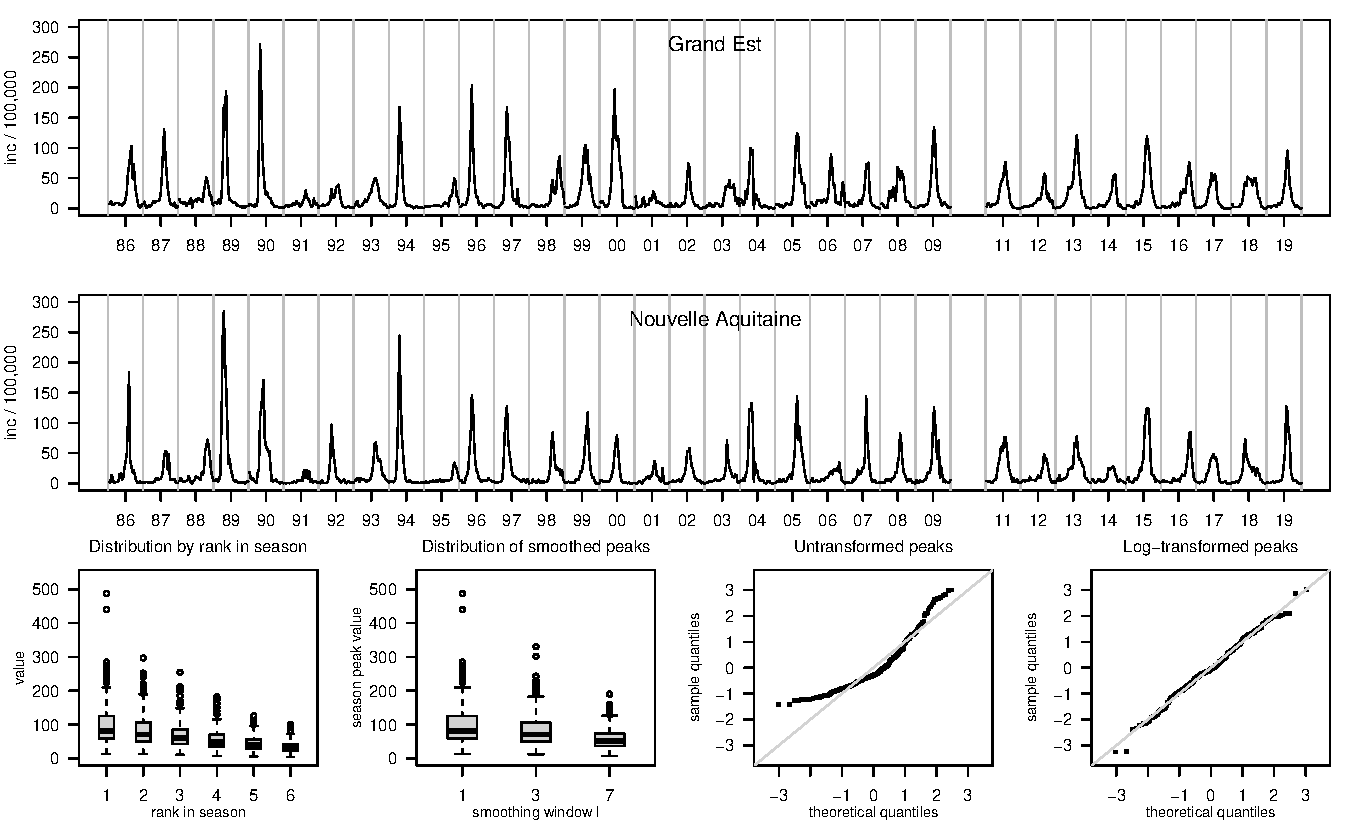
\includegraphics[width=1\textwidth]{figure/plot_data_fr.pdf}
\caption{Time series of weekly ILI cases per 100,000 population in the French regions of Grand Est and Nouvelle Aquitaine, 1985--2019. Off-season weeks are omitted in the plot, with grey lines delimiting the different seasons. The bottom row shows descriptive plots of the distribution of season peaks. First: Boxplots of incidence values by rank within season. Second: Boxplot of smoothed peak values as a function of the smoothing window width $l$. Third: Normal QQ plot of untransformed peak values. Fourth: Normal QQ plot of log-transformed peak values.}
\label{fig:data}
\end{figure}

\subsection{Results based on French data}

\subsubsection{Choice of transformation $f$ and number $n$ of observations used per season}

Figure \ref{fig:results1} summarizes thresholds resulting from different combinations of transformation function $f$ and number $n$ of observations used per season (specifications a--d from Section \ref{subsec:simulation_setup}). For each case we show mean thresholds, along with the empirical 5\% and 95\% quantiles, and the shares of new seasons classified into the different categories. This is complemented with summaries of the sensitivity, specificity and positive predictive value. All results are shown as a function of the number $m$ of historical seasons used. Where applicable, analytical approximations are shown as lines. These have been computed using equations \eqref{eq:expectation_q2} (with empirical means and covariances plugged in) and \eqref{eq:sens}--\eqref{eq:ppv}.

\begin{figure}[h!]
\centering
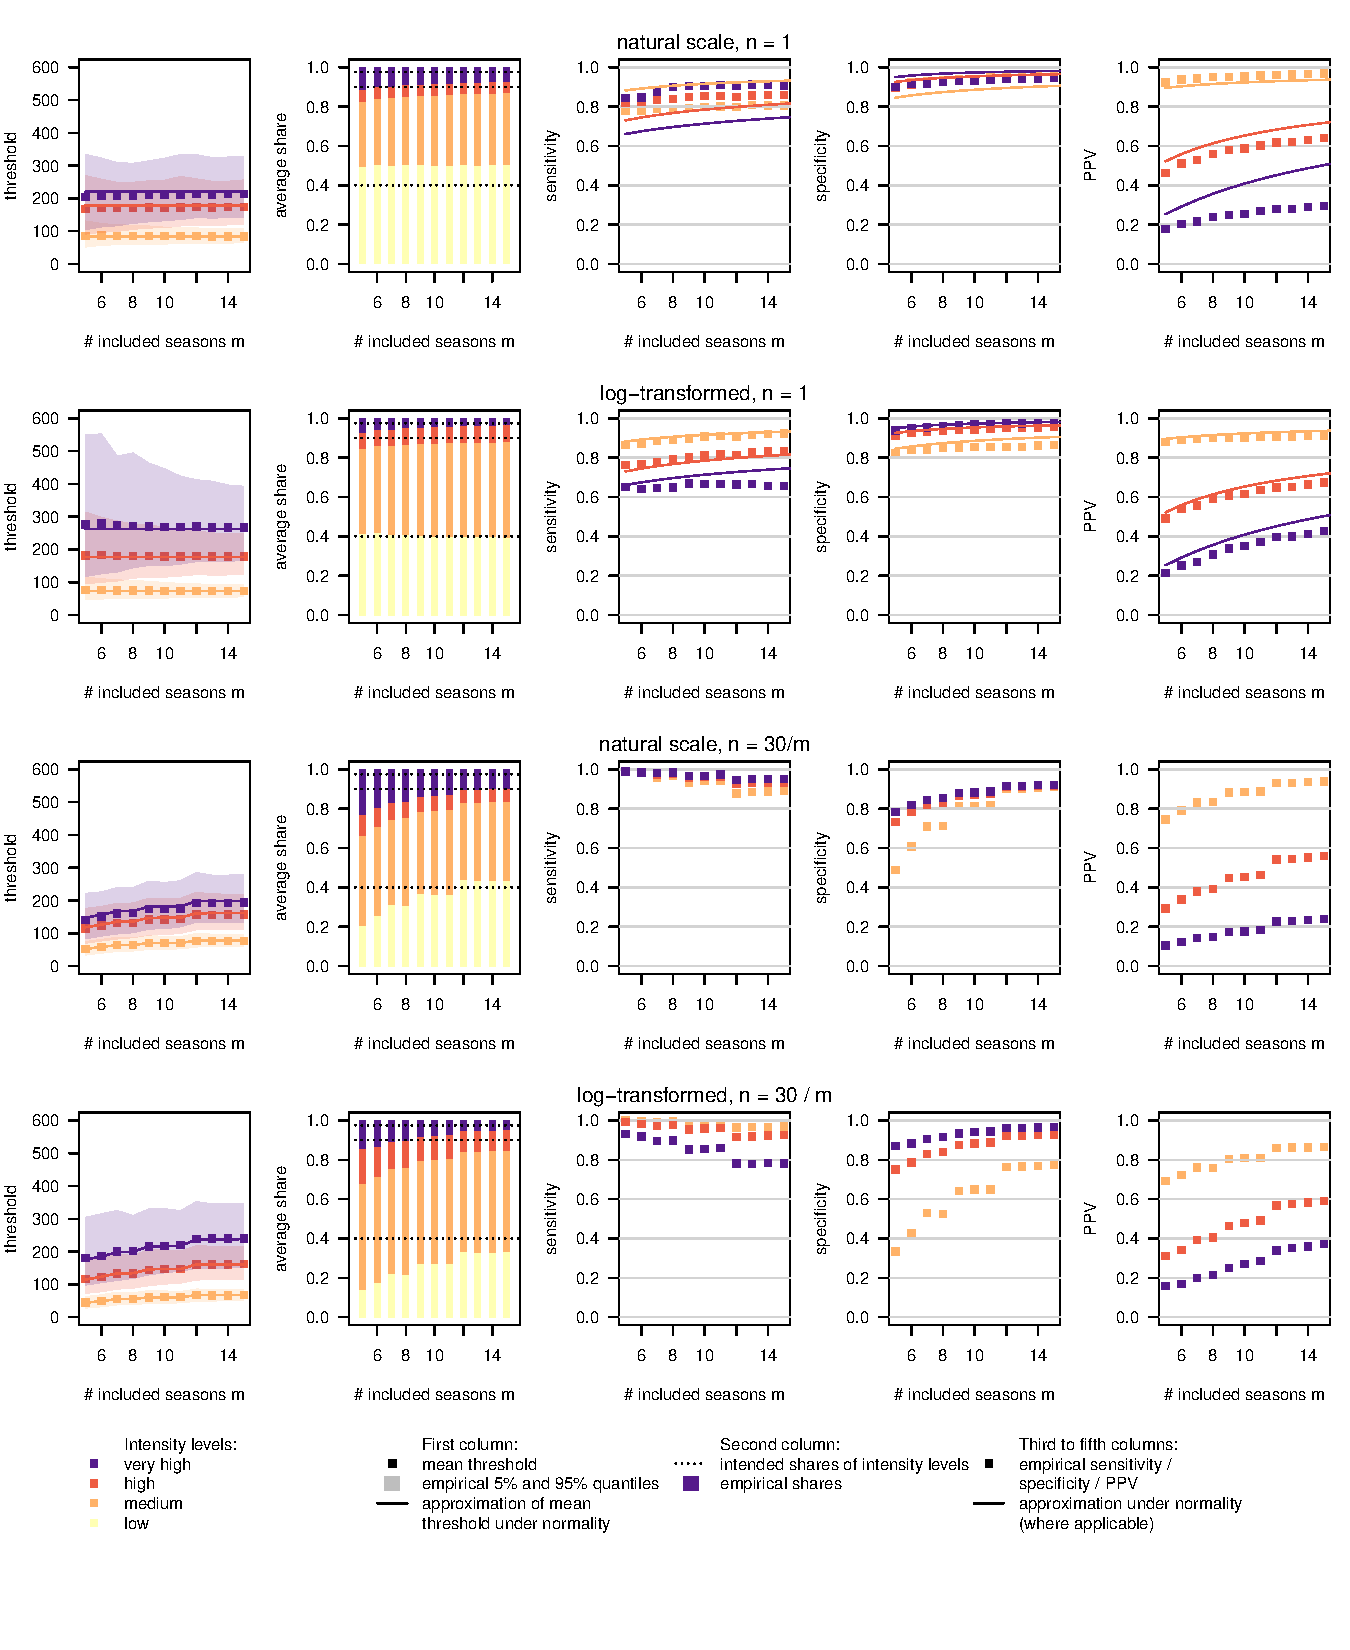
\includegraphics[width=1\textwidth]{figure/plot_fr.pdf}

\vspace{-1.5cm}

\caption{Impact of the choice of $n$ and transformation function $f$. First column: simulation-based mean intensity thresholds (squares) along with bands delimited by the empirical 5\% and 95\% quantiles. Analytical approximations of mean threshold values (computed from empirical means and covariances) are displayed as lines. Second column: resulting average shares of season peaks classified as low, medium, high and very high intensity. Third to fifth columns: sensitivity, specificity and PPVs of the different thresholds. Simulation results are shown as squares. Where available analytical approximations are shown as lines.}
\label{fig:results1}
\end{figure}

\textbf{Thresholds and threshold exceedance.} Thresholds for high and very high intensity are higher when a log transformation is employed. This leads to better calibration, i.e., the shares of seasons exceeding the high or very high thresholds are closer to the intended levels of 10\% and 2.5\%. Indeed, when using $n = 1$ observation per season and $m \geq 10$ historical seasons, the thresholds based on log-transformed data have very close to nominal exceedance rates. Without this transformation, new season peaks are classified as very high in roughly 10\% rather than 2.5\% of the cases. This indicates that the normal assumption is more appropriate after log tansformation, an aspect that already became visible from the normal QQ plot in Figure \ref{fig:data}.

As implied by the reasoning from Section \ref{subsec:choice_n}, letting the number of observations used per season depend on the number of available seasons via $n = 30/m$ leads to average thresholds which increase in $m$. When using a log transformation, they increase from 180 for $m = 5, n = 6$ to 218 for $m = 10, n = 3$ and 140 for $m = 15, n = 2$. For $n = 1$, in which case thresholds can be interpreted as unbiased (Section \ref{subsec:choice_n}), the average is around 270 and largely independent of $m$. Including historical observations which are not actual peaks thus leads to a considerable lowering of alarm thresholds and increases the number of alerts for high and very high influenza activity. For $m = 5, n = 6$ the proportion of seasons classified as very high is 15\% if a log transformation is used and 24\% otherwise. As can be seen from the fourth column, this is due to poor specificity, and as shown in the fifth column, leads to low positive predictive values. In the most extreme case where $m = 5$ seasons are used without a transformation, only one in ten seasons classified as very high is actually from the 2.5\% most extreme seasons. We note, however, that even the most well-behaved specification with $n = 1$ and a log transformation only yields a PPV slightly above 20\% for $m = 5$. For $m = 15$ this value roughly doubles. Our theoretical approximation is well aligned with the simulation results here (but much less so if no log transformation is used, as in this case the normality assumption is poorly fulfilled).


It can be noted that the thresholds generally have high variability (see the shaded bands in the first column of Figure \ref{fig:results1}). This is particularly pronounced for the very high threshold, and even more so if a logarithmic transformation is used. This reflects the general difficulty of estimating extreme quantiles from a small number of observations.

\textbf{Confusion matrices.} To complement these results and provide some more intuition on the intensity classifications, Figure \ref{fig:mosaic} shows confusion matrices for thresholds computed with a log transformation and different values of $m$. This represents a more detailed breakup of the results from the second column of Figure \ref{fig:results1}. Note that the perspective differs somewhat from the computation of sensitivities and specificities. There, we focused on \textit{threshold exceedance}, considering for instance whether the medium threshold was exceeded or not by a peak which was truly at least medium intensity. For the sensitivity of the medium threshold we thus ignored whether a peak which was truly medium intensity also exceeded the high threshold (which was in turn reflected in the specificity of the high threshold). Now we consider not just threshold exceedance, but the exact categorization. This is shown stratified by the true category of a peak, determined via the empirical distribution of all peaks (the highest 2.5\% are considered very high, the next 7.5\% high, the next 50\% medium and the remaining 40\% low).

For $n = 1$ (top two rows) it can be seen that in all categories misclassifications occur, but become somewhat less frequent for larger $m$. The log transformation yields better classification of truly medium and high peaks, while for truly low or very high peaks results are better without a transformation. This essentially reflects the fact that thresholds are more spaced out when using a log transformation (see Figure \ref{fig:results1}), giving medium and high peaks a better chance of correct classification. The rather modest positive predictive values from Figure \ref{fig:results1} are here reflected by the fact that in most panels, a large part of the peaks classified as very high (purple rectangles) are actually high or medium.

For $n = 30/m$, the miscalibration issues identified previously are again visible. For $m = 5$ and with a log transformation, more than 60\% of truly low peaks are classified as medium; roughly 40\% of medium peaks are classified as high or very high; and close to 75\% of high peaks are classified as very high. Similar pictures arise for thresholds computed on the natural scale, while as implied by theory, the problem is diminished with increasing $m$.

\begin{figure}
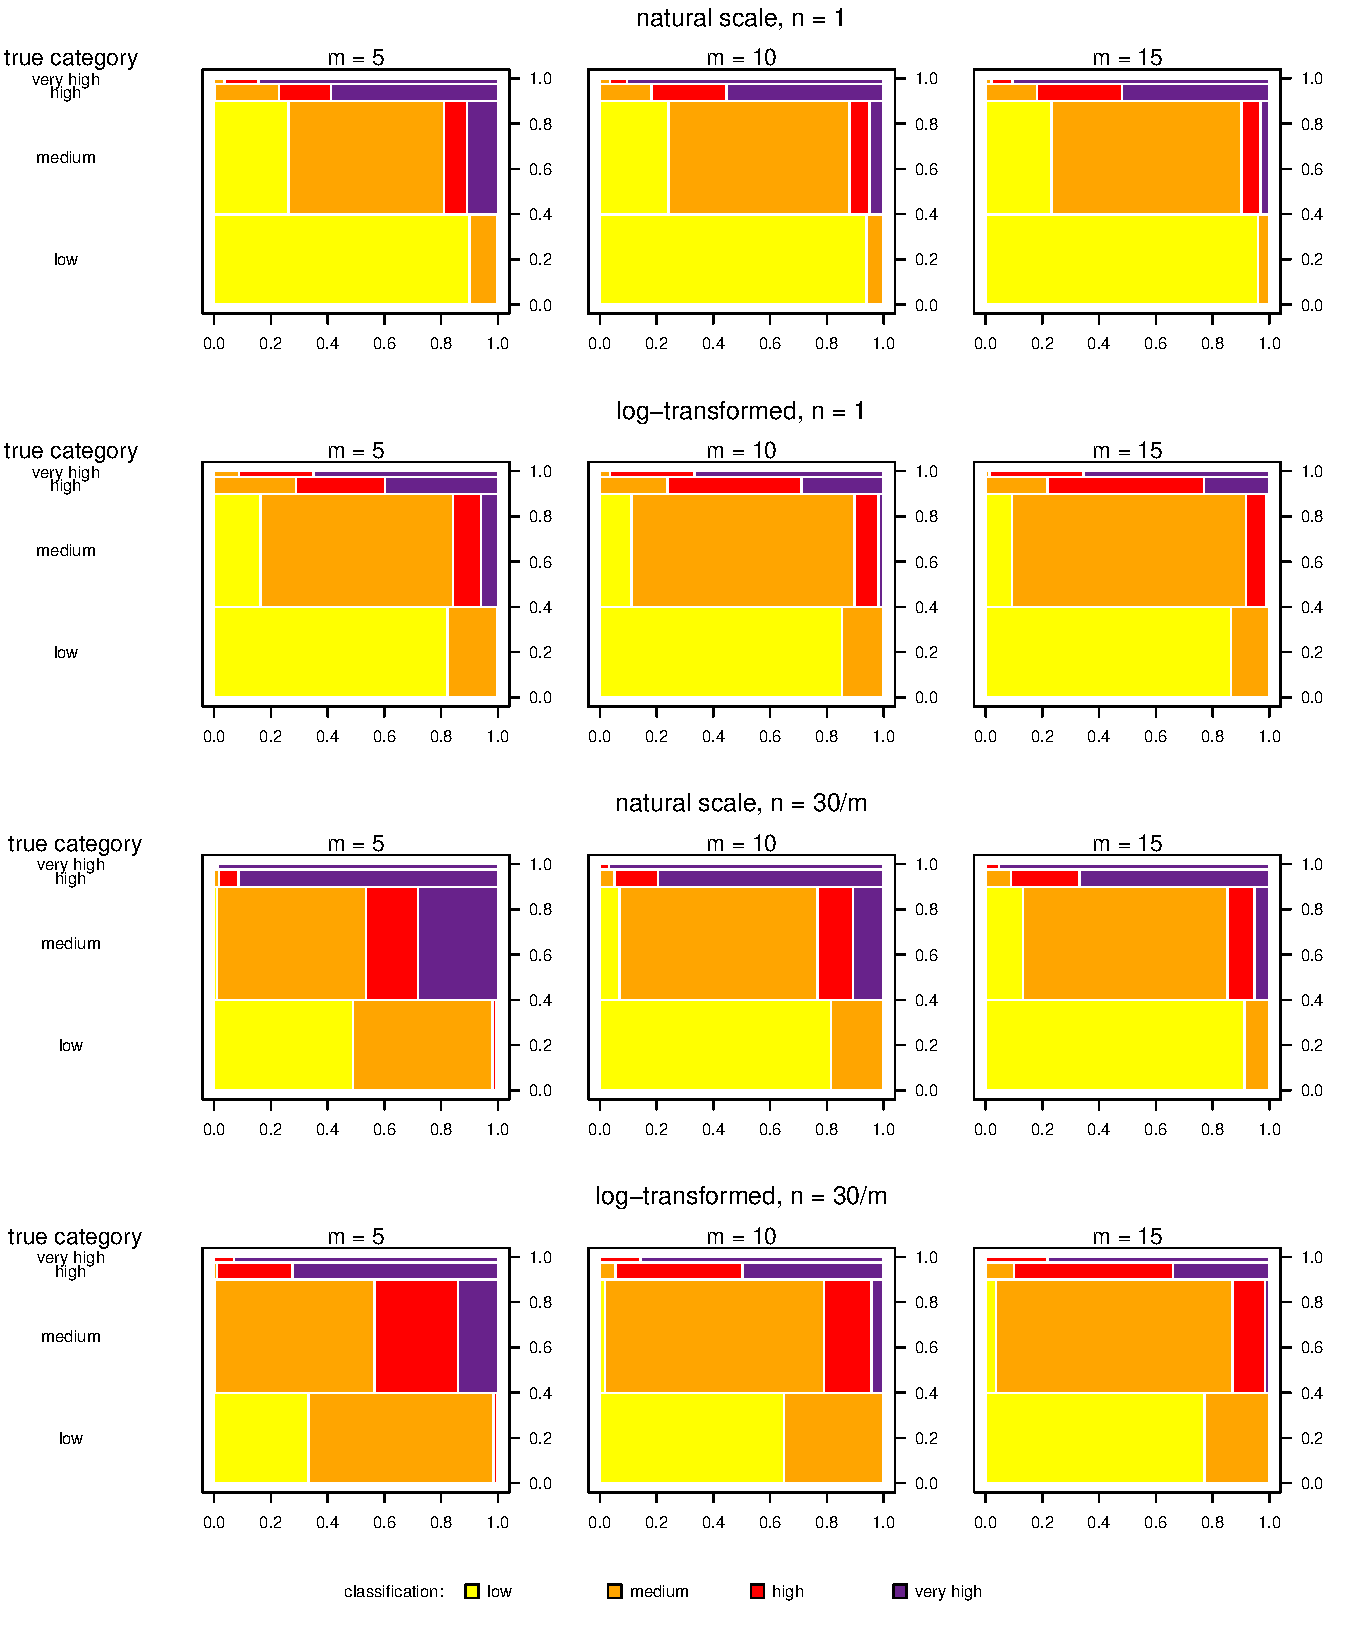
\includegraphics[width=0.9\textwidth]{figure/mosaic_fr.pdf}
\caption{Confusion matrices for intensity classifications obtained with different choices of $n$ and transformation function $f$. Mosaic plots show which fractions of season peaks which are truly very high, high, medium or low are classified into the four categories. The true class is determined with respect to the empirical quantiles of the distribution of peaks: very high (highest 2.5\% of all peaks), high (next 7.5\%), medium (next 50\%), low (lowest 40\% of all peaks).}
\label{fig:mosaic}
\end{figure}

% When always using $n = 1$, the average thresholds and shares of the different categories are more well-behaved also for small $m$. This holds especially when applying a log transformation, even though certain mismatches with the nominal exceedance probabilities remain. Also, there is considerable variability in the estimated thresholds (shaded areas in Figures \ref{fig:results1} and \ref{fig:results2}). These difficulties, however, are inherent in the problem of estimating a 90\% or 97.5\% quantile based on 5--10 observations.

% The increase of thresholds obtained with $n = 30/m$ as more historical data accumulate is not only a statistical tendency. For all four countries, the probability that the threshold for high intensity increases when using the first ten rather than only the first five years of a sampled sequence was around 90\%. For illustration of this aspect, consider the following example: We repeat a sequence of five ILI seasons from France (2014--2019) four times to obtain a time series of twenty seasons. We then apply the moving epidemic method with log transformation and $n = 30/m$ using the first $m = 5, 6, \dots, 20$ years of data, mimicking the development of thresholds as more historical data become available. As can be seen from the top panel of Figure \ref{fig:example_france}, this results in gradually increasing thresholds, despite the fact that the data in each five-year block behave the same. For example, season 6 is classified as very high intensity, but seasons 11 and 16 are not, even though they are identical to season 6 and the respective data used to construct thresholds follow exactly the same patterns. The bottom panel shows results obtained for the same time series with $n = 1$. While thresholds fluctuate quite a bit (with fluctuations dampening as the time series gets longer), there is no systematic trend.



%\begin{figure}
%\center
%\includegraphics[scale=0.6]{figure/example_france.pdf}
%\caption{Toy example to illustrate increasing thresholds as historical data accumulates: Data from France, 2014/2015--2018/2019 are appended three times and thresholds are computed using $m = 5, \dots, 15$ years of training data. The thresholds based on years 1 through $m$ are overlaid with the incidence time series from the $(m + 1)$-th year.}
%\label{fig:example_france}
%\end{figure}

\subsubsection{Smoothing of time series prior to computing thresholds}
\label{subsec:sim_smoothing}

\textbf{Thresholds and threshold exceedance.} We next assess the impact of smoothing historical data prior to computing thresholds (specifications e--f from Section \ref{subsec:simulation_setup}). Results for a window size of $l = 3$ and including a log transformation are shown in Figure \ref{fig:results_smoothing}. The top row shows the case where thresholds are applied to unsmoothed new peak values. In accordance with the theoretical arguments from Section \ref{subsec:smoothing}, the high and very high thresholds are exceeded more frequently than intended. When applying thresholds to smoothed new observations, the empirical and nominal exceedance levels are in good agreement. We note that thresholds are somewhat less variable than without smoothing, which we consider a desirable feature. As predicted by theory, sensitivity, specificity and positive predictive values are largely the same as without smoothing (compare the second rows of Figures \ref{fig:results1} and \ref{fig:results_smoothing}). While they are slightly higher in the present case we are unsure whether this will be the case in general. We provide a display for a stronger smoothing with $l = 7$ in Supplementary Figure \ref{fig:results_smoothing7}. If the resulting thresholds are applied to new unsmoothed peaks, more than a fifth of them is classified as very high intensity.

\begin{figure}[h!]
\centering
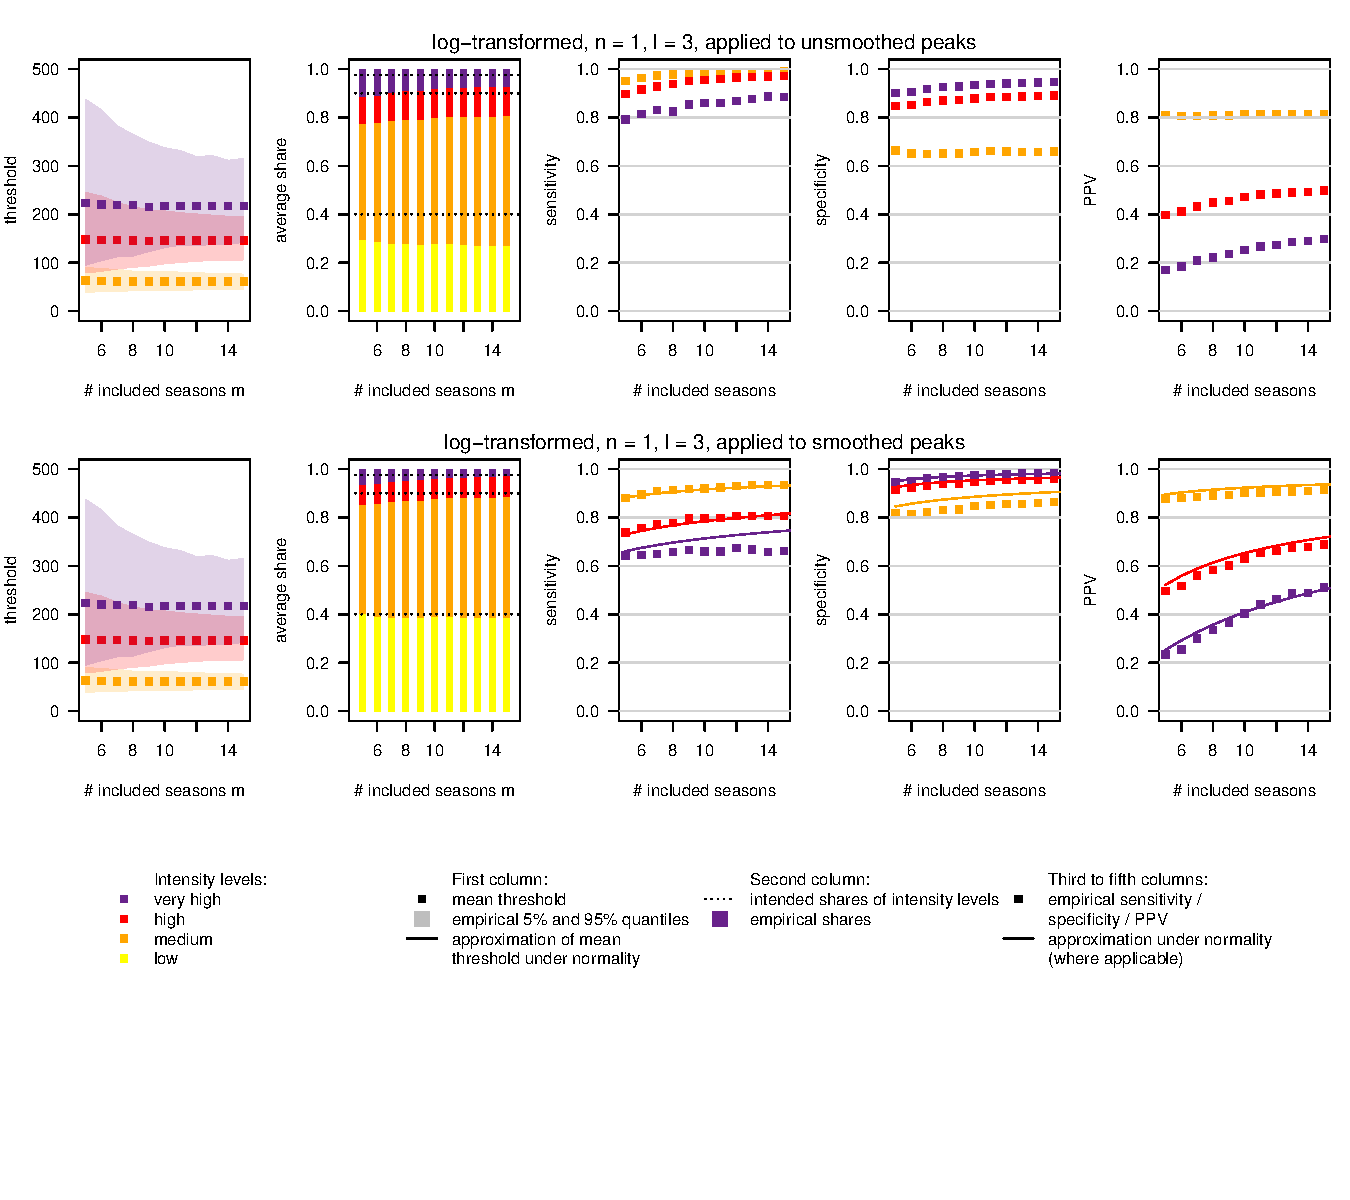
\includegraphics[width=1\textwidth]{figure/plot_smoothing3_fr_small.pdf}
\vspace{-33mm}

\caption{Impact of smoothing of historical data on thresholds. We applied a moving average with $l = 3$ to the historical time series prior to computing thresholds and subsequently applied them to either unsmoothed or smoothed new peak values. Results are shown for thresholds computed with a log transformation. See the caption of Figure \ref{fig:results1} for details on the plot elements.}
\label{fig:results_smoothing}
\end{figure}


\textbf{Confusion matrices.} We complement this again with confusion matrices, shown in Figure \ref{fig:mosaic_smoothing}. When unsmoothed new peaks are classified based on thresholds computed with smoothing, peaks tend to be assigned to too high categories. When thresholds are applied to smoothed new peaks, the results strongly resemble those obtained without smoothing of either historical or new peaks (compare second row of Figure \ref{fig:mosaic}).


\begin{figure}[h!]
\begin{center}
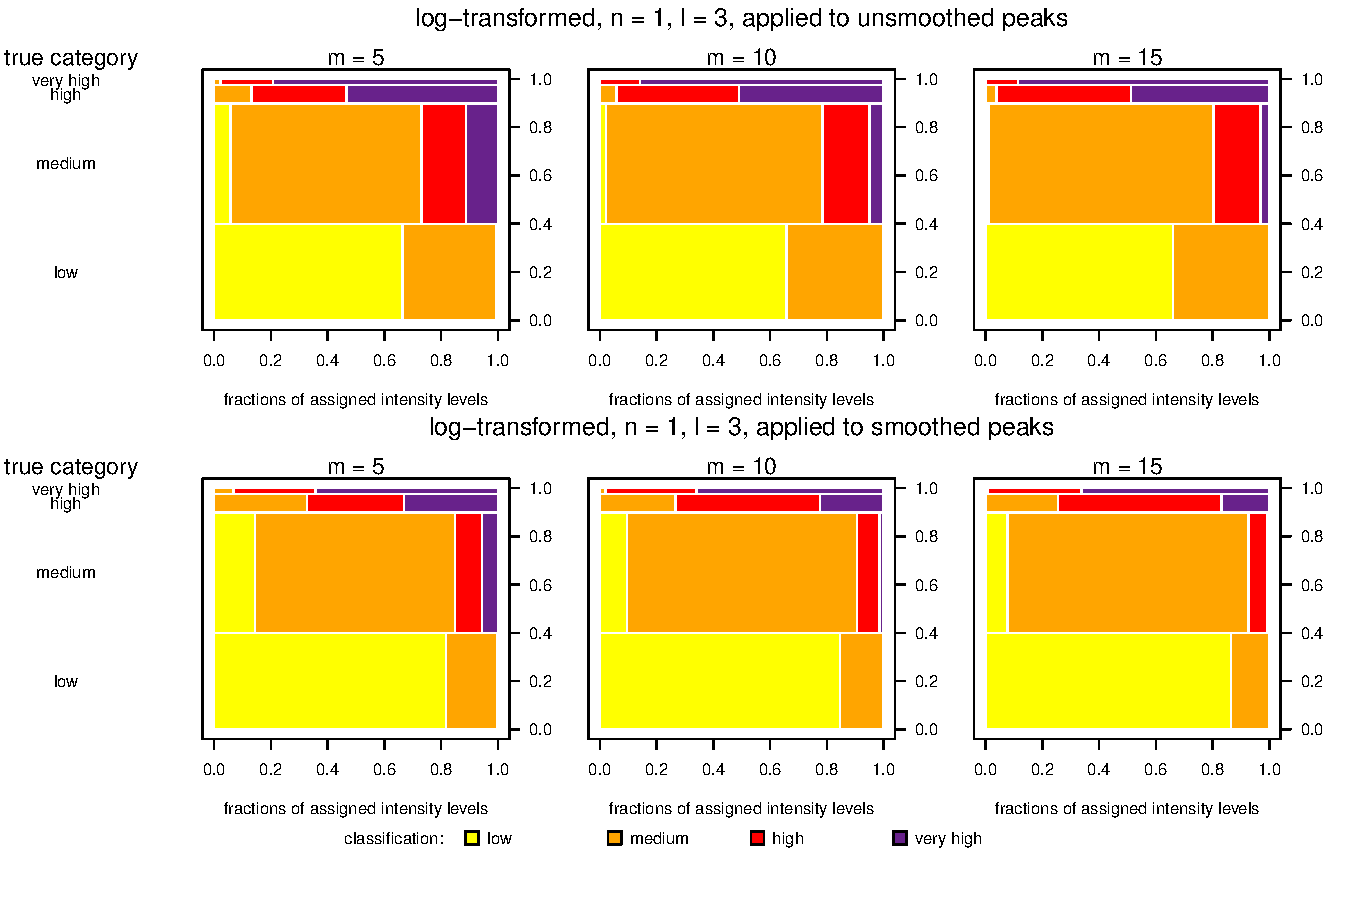
\includegraphics[width=0.9\textwidth]{figure/mosaic_log_smoothed_fr.pdf}
\caption{Confusion matrices for intensity classifications obtained with a smoothing window of width $l = 3$ and a log transformation. Top: thresholds applied to unsmoothed new peaks; bottom: thresholds applied to smoothed new peaks. Mosaic plots show which fractions of season peaks which are truly very high, high, medium or low are classified into the four categories, see camption of Figure \ref{fig:mosaic} for details.}
\end{center}
\label{fig:mosaic_smoothing}
\end{figure}


\subsubsection{Basing thresholds on confidence intervals}

Lastly we address thresholds based on confidence intervals (specifications g--h from Section \ref{subsec:simulation_setup}). As mentioned in Section \ref{subsec:cis} these are not the default in any of the  considered methods. However, they are implemented in the \texttt{mem} R package and due to terminological imprecisions in previous methods descriptions may be used by analysts programming their own routines. Figure \ref{fig:cis} shows that these thresholds are not well-behaved. As our theoretical reasoning suggested, the mean thresholds at different levels approach each other as $m$ grows. Overall, a considerably too large number of seasons is classified as very high intensity.

\begin{figure}[h!]
\begin{center}
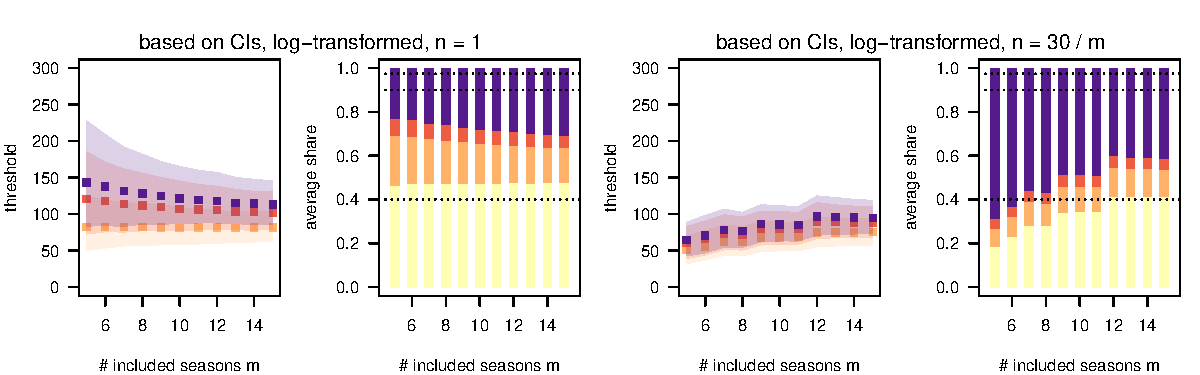
\includegraphics[width=0.9\textwidth]{figure/plot_ci_fr.pdf}
\end{center}
\caption{Average thresholds and exceedance shares when thresholds are based on confidence intervals rather than prediction intervals. See the caption and legend of Figure \ref{fig:results1} for details on the plot elements.}
\label{fig:cis}
\end{figure}

\subsection{Short summary of results based on US data}
\label{subsec:results_us}

The results obtained using the US data are overall very well aligned with those presented for the France in the previous sections. While there are of course some differences in the exact values of exceedance probabilities, sensitivities etc., the overall patterns and conclusions are identical. The agreement with the analytical approximations even tends to be better for the US data. % We take this as a sign of robustness of our findings.

\section{Discussion}
\label{sec:discussion}

\subsection{Practical recommendation}

We provided a statistical assessment of implementation choices in a widely used framework for the computation of influenza intensity thresholds. Our practical recommendation in light of the theoretical and empirical findings is as follows. We suggest including just one observation per season into the reference set and employing a log transformation. To make thresholds somewhat less variable, data can be smoothed using a moving average with $l = 3$. If smoothing is applied the resulting thresholds should be applied to new data smoothed using the same procedure. % We found that log transforming incidences prior to the computation of thresholds led to better behaved thresholds and closer to nominal exceedance rates. Concerning the question of how many observations per historical season should be included to compute thresholds, we found that the common choice $n = 30/m$ results in too low thresholds when few historical seasons are available. We therefore recommend adopting $n = 1$ irrespective of the number of available historical seasons. This is possible in the \texttt{R} package \texttt{mem} by setting \texttt{i.n.max = 1} when the function \texttt{memmodel} is called. Smoothing historical data prior to the computation of thresholds leads to somewhat less variable thresholds. However, it is important that the same smoothing procedure is also applied to new data before classifying the peak intensity. Otherwise a too large number of thresholds is classified as high or very high. We discourage the use of thresholds based on confidence intervals as they lead to an excessive number of seasons being classified as ``very high''.

\subsection{Further conclusions and outlook}

For a more detailed conclusion we return to the criteria evoked in Section \ref{sec:desirable_properties}.

\begin{description}
\item \textbf{Calibration.} The key to well-calibrated thresholds is that the observations in the reference set need to be comparable to new season peaks. This implies that no historical non-peak values should be included (i.e., one should choose $n = 1$). Otherwise thresholds will be pulled downwards and exceeded too frequently by new peaks. If historical data are smoothed ($l > 1$), comparability should be ensured by applying the same smoothing to new season peaks. Otherwise thresholds will again tend to be exceeded too often. Empirically we found that thresholds computed on log-transformed observations were better calibrated; while further study is needed we expect this to translate to other settings as distributions of peak values are typically skewed.
\item \textbf{Sensitivity and specificity.} Our theoretical and empirical results show that even if all assumptions are fulfilled, sensitivity and positive predictive values cannot be expected to exceed rather modest levels if $m$ is small. This aspect is unaffected by whether smoothing is applied or not and reflects the general difficulty of estimating extreme quantiles from few historical observations. Especially for the very high threshold at $\alpha = 0.975$, sensitivity and the PPV must be expected to be limited and it can be asked whether these thresholds are practically meaningful. In any case it does not seem advisable to add even more extreme thresholds to the procedure. This problem is in theory reduced if many historical seasons are available, but in practice there is a tradeoff with the recency and comparability of these data. If there are relelvant temporal trends or changes in surveillance systems, historical data may get outdated and their inclusion may not be helpful.
\item \textbf{Stability.} The same difficulties limiting the sensitivity and PPV imply that thresholds must be expected to be rather variable if $m$ is small. Empirically we found that this is even more the case if a log transformation is employed. Smoothing of historical data helps to somewhat reduce the variability of thresholds (but without improving sensitivity or specificity).
\item \textbf{Simplicity.} From a theoretical statistical standpoint the MEM and WHO methods are rather straightforward. However, informal exchange with users from public health indicates that given the large number of possible configurations, both methods are perceived as complex by practitioners. Our subjective opinion is that the methods overall strike a good balance here and that the demand for and practical benefits of more sophisticated methods may be limited. More specific guidance on how to choose the parameters of the methods and sensible default values are important to enable successful use of the methods.
\item \textbf{Ease of practical application.} Both methods can be applied using graphical user interfaces and thus do not require programming knowledge. For the MEM this is set up on top of an open-source R package with good documentation. For more technically versed users we recommend using this package directly. Combined with minimal data pre-processing it covers all aspects discussed in the present paper and enhances the automation and reproducibility of computations (which are the main challenge for graphical user interfaces).
\end{description}


% Our theoretical and empirical results highlight the general difficulty of estimating extreme quantiles of distributions from few historical observations. Even if the underlying assumptions are fulfilled, thresholds at $\alpha = 0.975$ will have modest positive predictive values. Inclusion of more historical seasons may help, but there is a tradeoff with the recency and comparability of these data. If there are relelvant temporal trends or changes in surveillance systems, historical data may get outdated and their inclusion may not be helpful. In light of these difficulties it can be asked whether the thresholds for very high incidence are practically meaningful. In any case it does not seem advisable to add even more extreme thresholds to the procedure.

In the present work we aimed to assess properties of the MEM and WHO methods in their current forms. However, a number of additional questions arise. Firstly, we focused purely on the assessment of season peak values, which is a useful perspective for temperate regions with one clear influenza wave per season. It could be discussed whether this should be complemented with other indicators and how more complex seasonal patterns as occuring in tropical regions should be handled. One possible alternative indicator is the season total, which conveys a different perspective on the severity of an influenza season. In this context we note that by smoothing an incidence time series prior to extracting peak values, we actually assess longer ``peak periods'', thus also changing the considered indicator. Which indicators are most relevant is a public health question and difficult to answer from a purely statistical standpoint; further exchange between the different subjects is thus needed. % Thresholds specific to each calendar week could also be defined (as is done e.g., in the Serfling method, see \citealt{Serfling1963}). Their interpretation, however, may be hampered by the strong variability in influenza season timing.

Another general question is whether a categorization into four categories is the most practical way of conveying influenza activity. In principle it would also be possible to just report the percentile of the fitted distribution corresponding to a new peak. This would result in a continuous scale from 0 to 100, with higher values indicating higher intensity. However, given the previously discussed difficulties with estimating extreme quantiles, a percentile-based display may also convey a false sense of exactness.

A more technical question concerns how extreme seasons in the historical data should be handled. These can have a substantial effect on thresholds. In our simulation study we pragmatically removed observations from the pandemic season 2009/2010. However, a more principled approach to determining which historical seasons should be excluded would be desirable. As the same problem arises in outbreak detection, this strand of literature may be a helpful starting point (see e.g., \citealt{Noufaily2013}).



A limitation of our simulation study is that the re-sampled data do not actually stem from one and the same time series, but from several different regions. This made some re-scaling necessary. After log transformation, the resulting reference set is well-described by a normal distribution, but it is unclear how generalizable this is. A strength of our re-sampling scheme is that it ensures a realistic correlation structure between season peaks and the surrounding values, which would be challenging to achieve with fully synthetic data. A weakness is that dependence structures across seasons are not preserved. For certain respiratory diseases, alternating patterns between intense and mild seasons are common, likely due to gradual waning of immunity. Such patterns may affect the behaviour of thresholds, but are removed from our simulation study. We re-ran all simulation studies using a smaller data set from the United States and obtained very similar results. We take this as a sign of robustness at least for temperate settings. Intensity thresholds in tropical regions pose specific challenges like seasons with multiple peaks, which we did not address in the present manuscript.



% We focused on the computation of influenza intensity thresholds, but the same general arguments apply to the computation of thresholds to determine the onset of a season \citep{Vega2012}. As variability among observations around the season onset may be lower than around the peak the problem may be less severe; we did not assess this empirically as not all our data sets fully covered the off-season.

To conclude, we re-emphasize the importance of a simple and interpretable thresholding method with a thorough open source software implementation like \texttt{mem}. The use of a standard approach will improve comparability of results and facilitate further methodological advances. With this work we hope to contribute to the development of best practices  with a statistical perspective, complementing public health practitioners' applied experience.


\section*{Data and code}

Materials to reproduce the presented results are available at \url{https://github.com/jbracher/mem_who}.

\section*{Ethics statement}

No ethics approval was necessary as this study uses exclusively publicly available data.


% \section*{Author contributions}

% Study concept: JB; Data processing: JB and JL; Literature review: JB and JL; Statistical analysis / implementation: JB; Writing and editing: JB and JL.


\section*{Acknowledgements}

We would like to thank Michael H\"ohle, Rob Moss, Laura Werlen and Daniel Wolffram for helpful discussions. Johannes Bracher was supported by the Helmholtz Foundation via the SIMCARD Information and Data Science Pilot Project as well as Deutsche Forschungsgemeinschaft (DFG, German Research Foundation) -- project number 512483310.

{\footnotesize
\bibliographystyle{apalike}
\bibliography{bibliography_mem}
}

\appendix

\section{Derivations of analytical approximations}
\label{appendix:derivations}

\subsection{Derivations for Section \ref{subsec:choice_n}}
\label{appendix:derivation_n}

We start by addressing the expectations of empirical mean $\bar{Y}$ and variance $S^2$ of the reference observations, where
\begin{align*}
\bar{Y} & = \frac{1}{mn} \sum_{j = 1}^m \sum_{i = 1}^n Y_i^{(j)}\\
S^2 & = \frac{1}{mn - 1} \sum_{j = 1}^m \sum_{i = 1}^n \left(Y_i^{(j)} - \bar{Y}\right)^2.
\end{align*}
It is straightforward to see that 
\begin{equation}
\mathbb{E}(\bar{Y}) = \frac{1}{n} \sum_{i = 1}^n \mu_i.
\end{equation}
For the variance $S^2$, we first note that it can be re-written as
\begin{align}
S^2 & = \frac{mn}{mn - 1} \left\{\frac{1}{mn} \sum_{j = 1}^m \sum_{i = 1}^n \left(Y_i^{(j)} - \bar{Y}\right)^2 \right\}\\
& = \frac{mn}{mn - 1} \left\{ \underbrace{\frac{1}{mn} \sum_{j = 1}^m \sum_{i = 1}^n Y_i^{(j)2}}_{\text{denote this by } a} \ \ \ - \ \ \ \underbrace{\left(\frac{1}{mn} \sum_{j = 1}^m \sum_{i = 1}^n Y_i^{(j)} \right)^2}_{\text{denote this by } b} \right\} \label{eq:sigma2hat}
\end{align}
%$$
%\sd^2 = \underbrace{\left(\frac{1}{nK - 1} \sum_{j = 1}^n \sum_{i = 1}^K Y_i^{(j)2}\right)}_{ = a} \ \ \ - \ \ \ \underbrace{\left(\frac{1}{nK - 1} \sum_{j = 1}^n \sum_{i = 1}^K Y_i^{(j)} \right)^2}_{= b}.
%$$
We consider the two terms $a$ and $b$ separately, starting by
\begin{align*}
\mathbb{E}(a) & = \frac{1}{mn} \sum_{j = 1}^m \sum_{i = 1}^n \mathbb{E}\left(Y_i^{(j)2}\right)\\
& = \frac{1}{mn} \sum_{j = 1}^m \sum_{i = 1}^n \left\{ \text{Var}\left(Y_i^{(j)}\right) + \mathbb{E}\left(Y_i^{(j)}\right)^2 \right\}\\
& = \frac{m}{mn} \sum_{i = 1}^n (\sigma_{i}^2 + \mu_i^2).
\end{align*}
Then we note that
\begin{align*}
\mathbb{E}(b) & = \mathbb{E}\left\{\left(\frac{1}{mn} \sum_{j = 1}^m \sum_{i = 1}^n Y_i^{(j)} \right)^2\right\}\\
& = \text{Var}\left( \frac{1}{mn} \sum_{j = 1}^m \sum_{i = 1}^n Y_i^{(j)} \right) \ \ \ + \ \ \ \mathbb{E}\left(\frac{1}{mn}  \sum_{j = 1}^m \sum_{i = 1}^n Y_i^{(j)} \right)^2\\
& = \frac{1}{(mn)^2}\sum_{j = 1}^m \text{Var}\left(\sum_{i = 1}^n Y_i^{(j)} \right) \ \ \ + \ \ \ \left(\frac{m}{mn} \sum_{i = 1}^n \mu_i\right)^2\\
& = \frac{m}{(mn)^2} \sum_{i = 1}^n \sum_{i' = 1}^n \sigma_{i,i'} \ \ \ + \ \ \ \frac{m^2}{(mn)^2}\left(\sum_{i = 1}^n \mu_i\right)^2.
\end{align*}
Plugging these results back into equation \eqref{eq:sigma2hat} we obtain
\begin{equation}
\mathbb{E}(S^2) = \frac{m}{mn - 1} \sum_{i = 1}^n (\sigma_{i}^2 + \mu_i^2) \ \ \ - \ \ \ \frac{1}{n(mn - 1)} \sum_{i = 1}^n \sum_{i' = 1}^n \sigma_{i,i'} \ \ \ - \ \ \ \frac{m}{n(mn - 1)}\left(\sum_{i = 1}^n \mu_i\right)^2.
\label{eq:expectation_sigma2_2}
\end{equation}
It is straightforward to see that for $n = 1$ the expressions \eqref{eq:expectation_mu} and \eqref{eq:expectation_sigma2_2} simplify to
$$
\mathbb{E}(\bar{Y}) = \mu_1 \ \ \text{ and } \ \ \mathbb{E}(S^2) = \sigma^2_1,
$$
as given in equation \eqref{eq:expectation_sigma2}.

There is no general way of computing the expectation $\mathbb{E}(S)$ from $\mathbb{E}(S^2)$, but unless the true distribution of  $S^2$ has strong excess curtosis,
\begin{equation}
\mathbb{E}(S) \approx \sqrt{\mathbb{E}(S^2)}
\label{eq:expectation_sigma}
\end{equation}
is a reasonable approximation. We can then plug equations \eqref{eq:expectation_mu} and \eqref{eq:expectation_sigma} into the formulae for the thresholds $q_{Y, \alpha}$ on the transformed scale and obtain
$$
\mathbb{E}(\hat{q}_{Y, \alpha}) \approx \mathbb{E}(\bar{Y}) + z_\alpha \sqrt{\mathbb{E}(S^2)},
$$
where $z_\alpha$ is the $\alpha$ quantile of the standard normal distribution (with $\alpha \in \{0.4, 0.9, 0.975\}$).

If $f$ was set to the natural logarithm, the question remains how to obtain statements concerning thresholds $q_{X, \alpha}$ on the original scale. Approximation via a second-order Taylor expansion yields
\begin{equation}
\mathbb{E}(\hat{q}_{X, \alpha}) = \mathbb{E}\left\{\exp(\hat{q}_{Y, \alpha})\right\} \approx \exp\left\{\mathbb{E}(\hat{q}_{Y, \alpha})\right\} \times \left\{1 + \frac{\text{Var}(\hat{q}_{Y, \alpha})}{2} \right\}.
\label{eq:taylor}
\end{equation}
Empirically, after transformation to the log scale, the variance of the reference observations is low in our applied setting. The resulting variances of $q_{Y, \alpha}$ are then quite small and do not play an important role in equation \eqref{eq:taylor}. We can thus use the even simpler approximation
\begin{equation}
\mathbb{E}(q_{\hat{Y}, \alpha}) \approx \exp\left\{\mathbb{E}(\hat{q}_{Y, \alpha})\right\} \approx \exp\{\mathbb{E}(\bar{Y}) + z_\alpha \sqrt{\mathbb{E}(S^2)}\}.
\end{equation}
As can be seen from Figures 2 and 3 from the main manuscript, this approximation works very well in practice. % To compute the values indicated by the small black crosses, we just plugged the empirical mean vectors and covariance matrices of the $\mathbf{Y}_j$ in the respective data sets into equations \eqref{eq:expectation_mu}--\eqref{eq:expectation_q}.

\subsection{Derivations for Section \ref{subsec:smoothing}}

Remember that we denote by $p_j$ the peak week of the smoothed incidences in season $j$ and defined
$$
x^\text{smo}_{j, p_j} = \sum_{d = 0}^l x^\text{raw}_{j, p_j - d} = \begin{pmatrix} 1/l \\ \vdots \\ 1/l \end{pmatrix}^\top \mathbf{X}^{\text{raw}}_j.
$$
As we assumed that $n = 1$ and $f$ is the identity function (i.e., $y_j^{(1)} = x_j^{(1)}$), equation \eqref{eq:moments} simplifies to
\begin{align}
\begin{split}
\bar{Y} & = \frac{\sum_{j = 1}^m x_{j, p_j}^\text{smo}}{nm}\\
S^2 & = \sqrt{ \frac{\sum_{j = 1}^m (x_{j, p_j}^\text{smo}  - \bar{y})}{nm - 1}}.
\end{split}
\end{align}
It is clear that
$$
\mathbb{E}(\bar{Y}) = \begin{pmatrix} 1/l \\ \vdots \\ 1/l \end{pmatrix}^\top \mathbb{E}(\mathbf{X}^{\text{raw} \top}_j) = \begin{pmatrix} 1/l \\ \vdots \\ 1/l \end{pmatrix}^\top \boldsymbol{\mu}^\text{raw} = \frac{1}{l}\sum_{i = 1}^l \mu^\text{raw}_i.
$$
The expression for $S^2$ is known to be an unbiased estimator for the variance of $X_{j, p_j}^\text{smo}$, i.e.
$$
\mathbb{E}(S^2) = \text{Var}(X_{j, p_j}^\text{smo}) = \begin{pmatrix} 1/l \\ \vdots \\ 1/l \end{pmatrix}^\top \mathbf{\Sigma}^\text{raw} \begin{pmatrix} 1/l \\ \vdots \\ 1/l \end{pmatrix} = \ \frac{1}{l^2} \sum_{i = 1}^l \sum_{i' = 1}^n \sigma^\text{raw}_{i', i}.
$$
This completes the proof.

\subsection{Derivations for Section \ref{subsec:theory_sensitivity}}

As the exceedance of thresholds is invariate to shifting and scaling of the $Y^{(i)}_j$ we can for simplicity assume that they follow a standard normal distribution with $\mu_1 = 0, \sigma^2_1 = 1$. Now consider
$$
\hat{q}_{Y, \alpha} = \bar{Y} + z_\alpha S.
$$
Basu's theorem tells us that the sample mean and standard deviation are independent. We can thus  address their respective distributions separately. We obviously have
$$
\bar{Y} \sim \text{N}\left(0, \frac{1}{m}\right).
$$
It is moreover known that for the sample variance $S^2$ of $m$ standard normal random variables
$$
[(m - 1) \times S^2] \sim \chi^2(m - 1)
$$
holds \citep{HELM2008}. The square root of a $\chi^2$ distributed random variable can be approximated well by a normal distribution \citep[p426]{Johnson1994}. Specifically, we get
$$
\sqrt{2 \times (m - 1) \times S^2} \ \  \stackrel{\text{approx}}{\sim} \ \ \text{N}(\sqrt{2m - 2}, 1)
$$
and thus
$$
S \ \  \stackrel{\text{approx}}{\sim} \ \ \text{N}\left(1, \frac{1}{2\times(m - 1)}\right).
$$
Combining these two results and using the independece of sample mean and standard deviation, we get
$$
\hat{q}_{Y, \alpha} \ \  \stackrel{\text{approx}}{\sim} \ \ \text{N}\left[z_\alpha, \frac{1}{m} + z_\alpha^2 \times \frac{1}{2 \times (m - 1)} \right].
$$
Equation \eqref{eq:q_Y} is then obtained by simple re-scaling and shifting.

We can now compute the sensitivity. It corresponds to the probability that $Y^{(1)}_{m + 1} > \hat{q}_{Y, \alpha}$ given exceedance $Y^{(1)}_{m + 1} > z_\alpha$ (keep in mind that $y^{(1)}_{m + 1}$ it is assumed to follow a standard normal distribution). This conditional probability is straightforward to evaluate using the integral in equation \eqref{eq:sens}. The derivation of the specificity follows the same argument.

\newpage

\section{Supplementary figure based on French data}

\begin{figure}[h!]
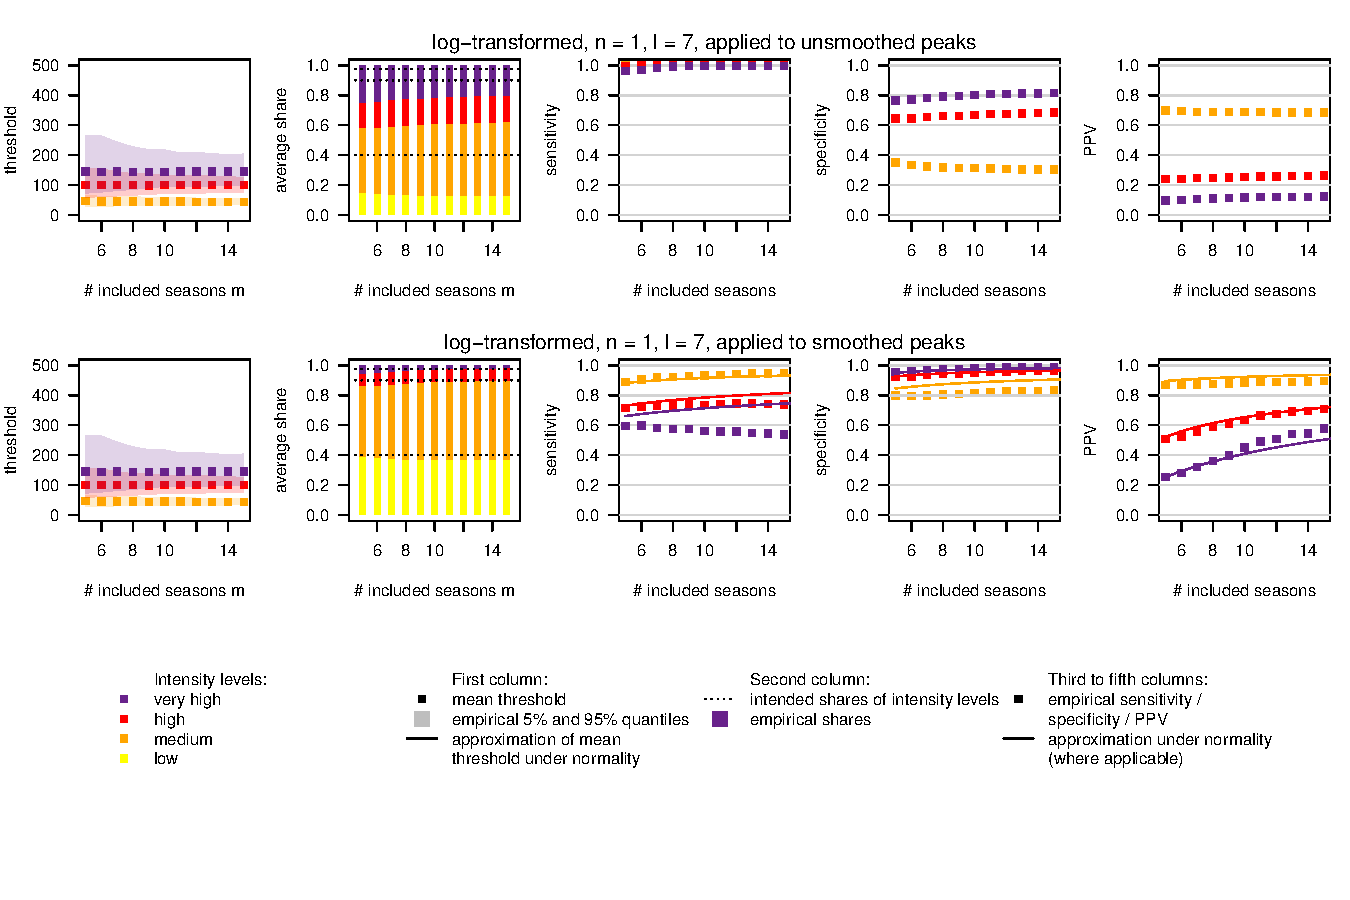
\includegraphics[width=0.95\textwidth]{figure/plot_smoothing7_fr_small.pdf}
\caption{Impact of smoothing of historical data on thresholds. We applied a moving average with $l = 7$ to the historical time series prior to computing thresholds and subsequently applied them to either unsmoothed or smoothed new peak values. Results are shown for thresholds computed with a log transformation. See the legend of Figure \ref{fig:results1} for details on the plot elements.}
\label{fig:results_smoothing7}
\end{figure}

\newpage

\section{Supplementary figures based on US data}
\label{suppl:us}

In the following, Figures \ref{fig:data}--\ref{fig:cis} are reproduced using the data from the US described in Section \ref{subsec:data}.

\begin{figure}[h]
\center
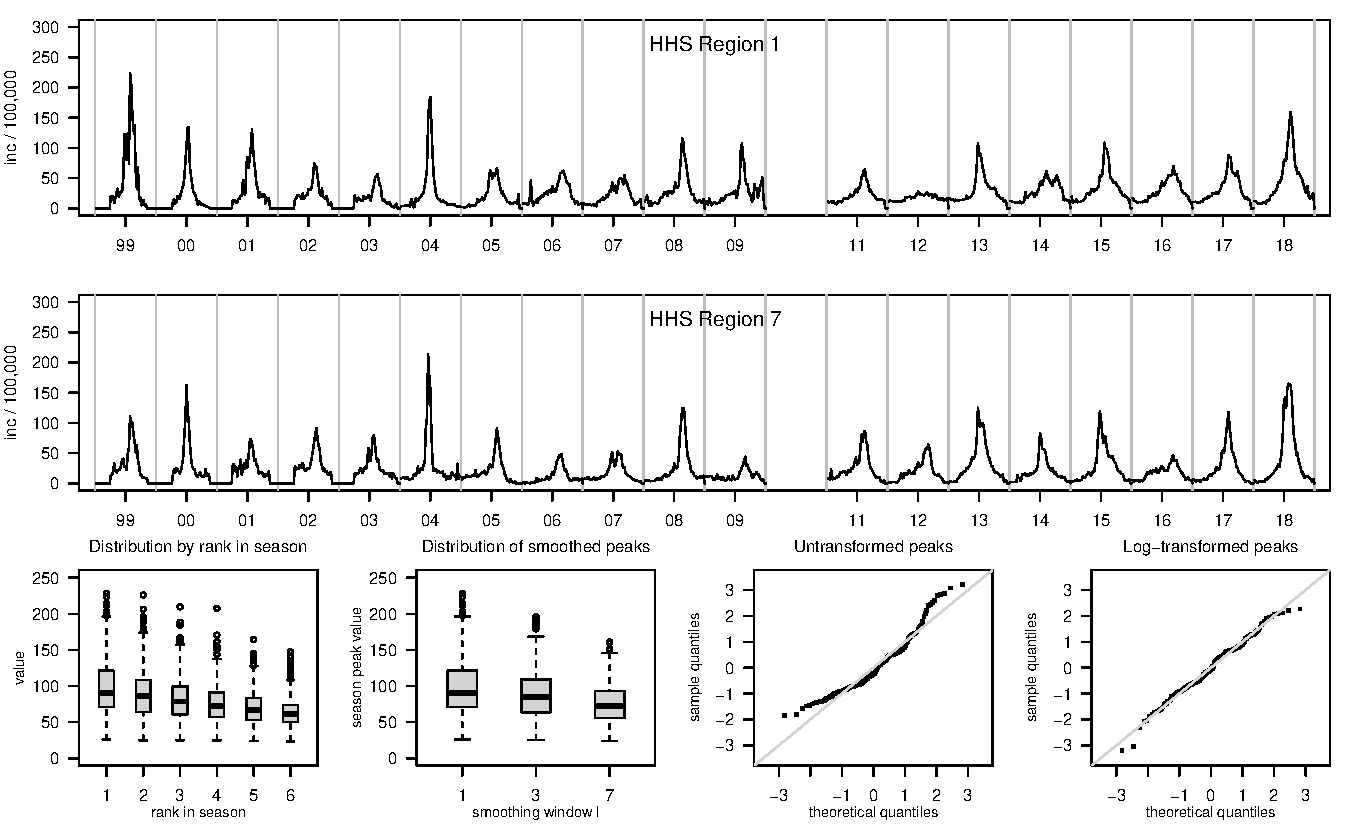
\includegraphics[width=1\textwidth]{figure/plot_data_us.pdf}
\caption{Reproduction of Figure \ref{fig:data} using US data. Time series of weekly weighted ILI percentages in US HHS Regions 1 and 7, 1999--2018. Off-season weeks are omitted in the plot, with grey lines delimiting the different seasons. The bottom row shows descriptive plots of the distribution of season peaks. First: Boxplots of incidence values by rank within season. Second: Boxplot of smoothed peak values as a function of the smoothing window width $l$. Third: Normal QQ plot of untransformed peak values. Fourth: Normal QQ plot of log-transformed peak values.}
\label{fig:data_us}
\end{figure}

\begin{figure}[h!]
\centering
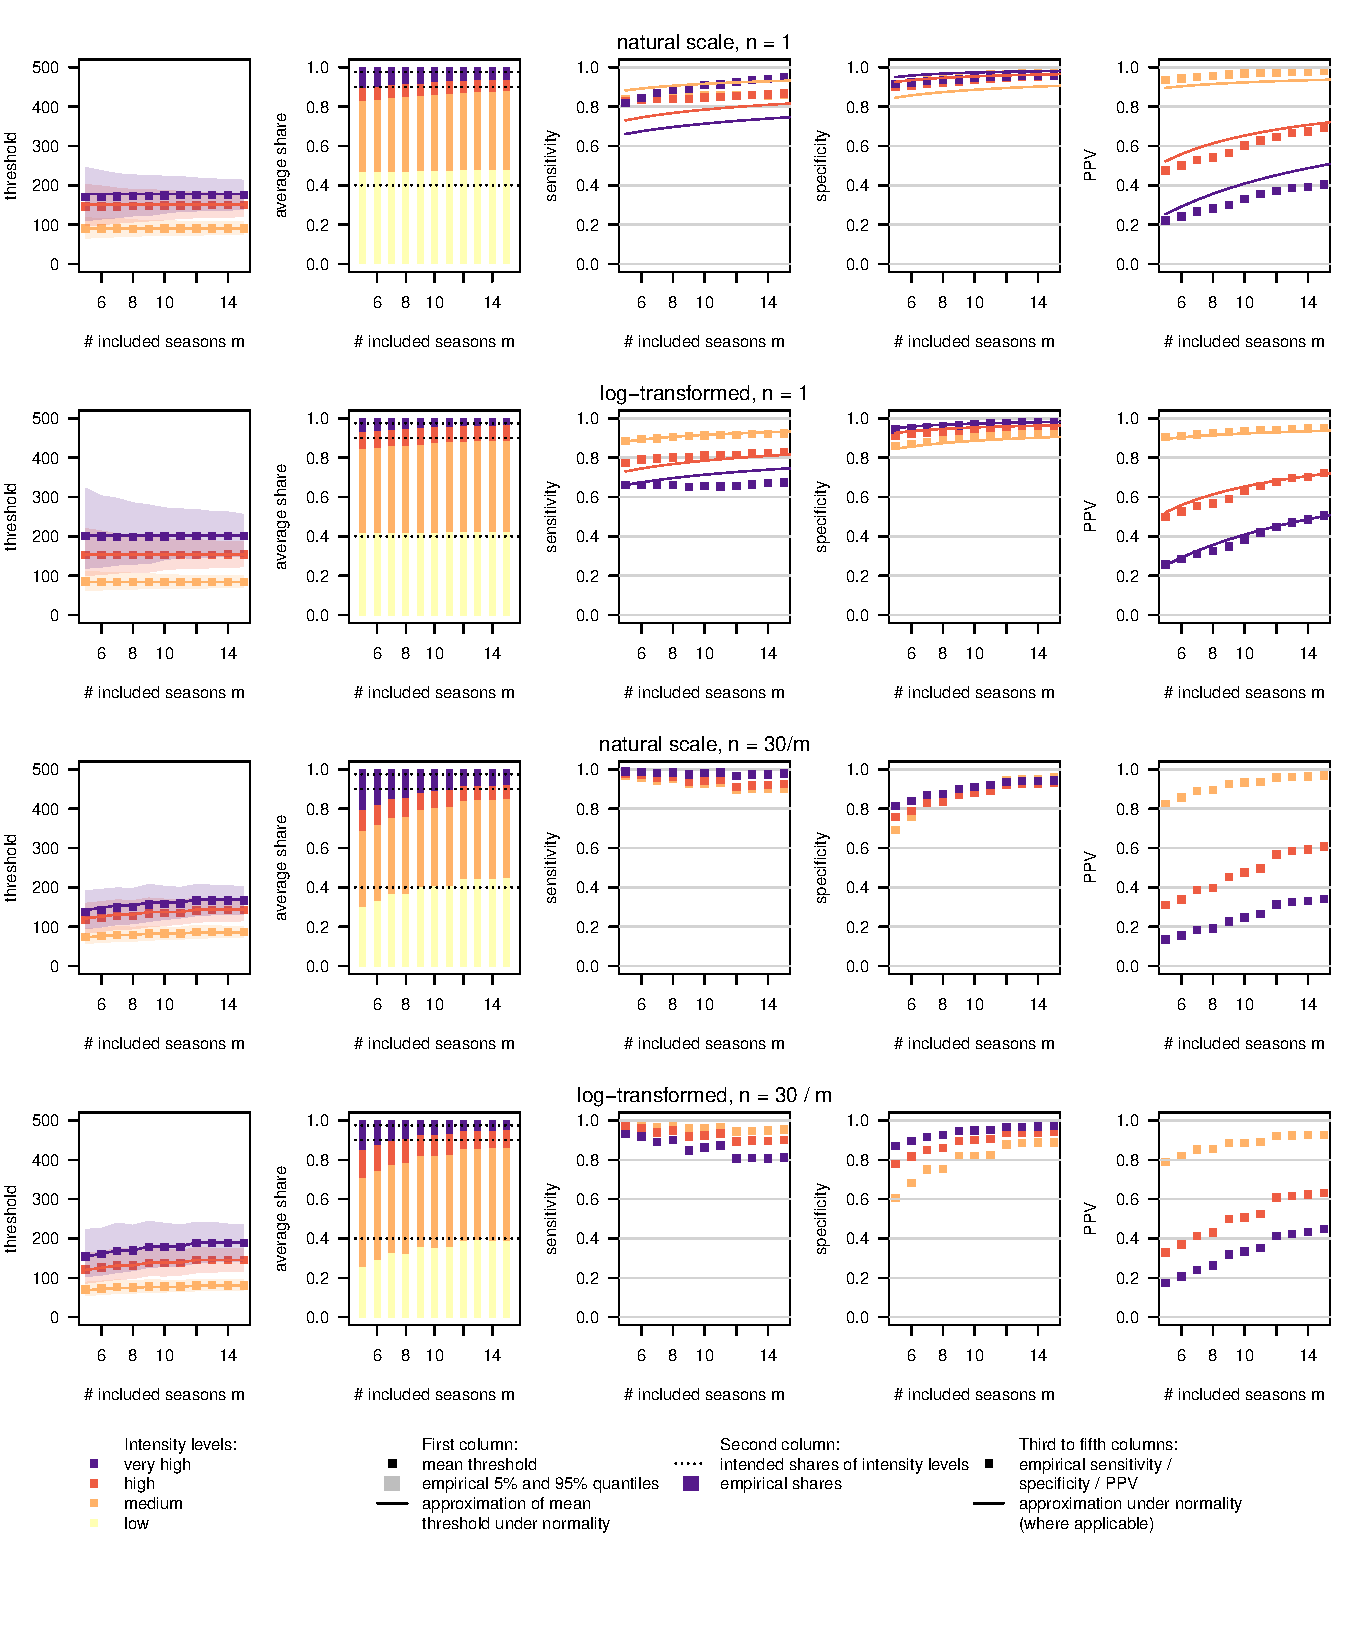
\includegraphics[width=1\textwidth]{figure/plot_us.pdf}

\vspace{-1.5cm}

\caption{Reproduction of Figure \ref{fig:results1} using US data. Impact of the choice of $n$ and transformation function $f$. First column: simulation-based mean intensity thresholds (squares) along with bands delimited by the empirical 5\% and 95\% quantiles. Analytical approximations of mean threshold values (computed from empirical means and covariances) are displayed as lines. Second column: resulting average shares of season peaks classified as low, medium, high and very high intensity. Third to fifth columns: sensitivity, specificity and PPVs of the different thresholds. Simulation results are shown as squares. Where available analytical approximations are shown as lines.}
\label{fig:results1_us}
\end{figure}


\begin{figure}
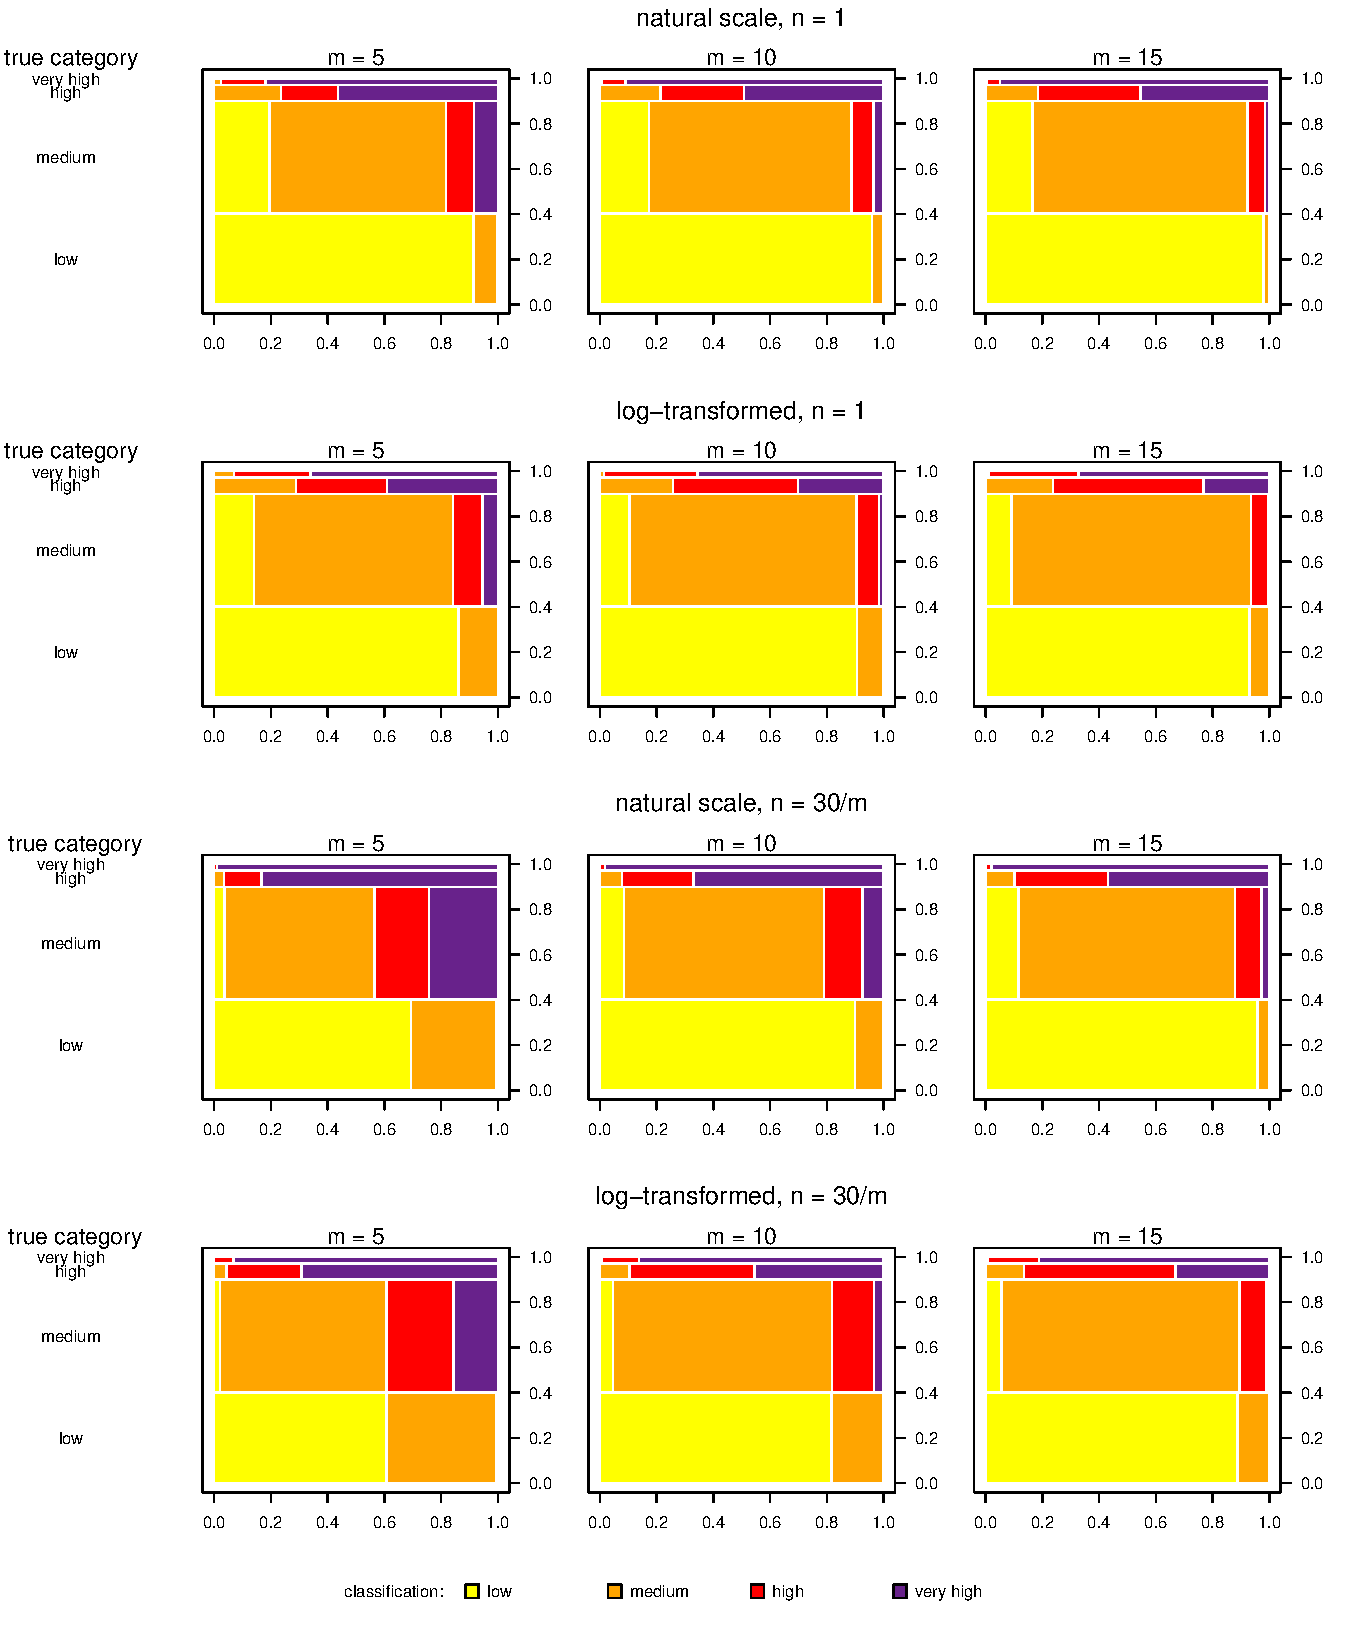
\includegraphics[width=0.95\textwidth]{figure/mosaic_us.pdf}
\caption{Reproduction of Figure \ref{fig:mosaic} using US data. Confusion matrices for intensity classifications obtained with different choices of $n$ and transformation function $f$. Mosaic plots show which fractions of season peaks which are truly very high, high, medium or low are classified into the four categories. The true class is determined with respect to the empirical quantiles of the distribution of peaks: very high (highest 2.5\% of all peaks), high (next 7.5\%), medium (next 50\%), low (lowest 40\% of all peaks).}
\label{fig:mosaic_us}
\end{figure}



\begin{figure}[h!]
\centering
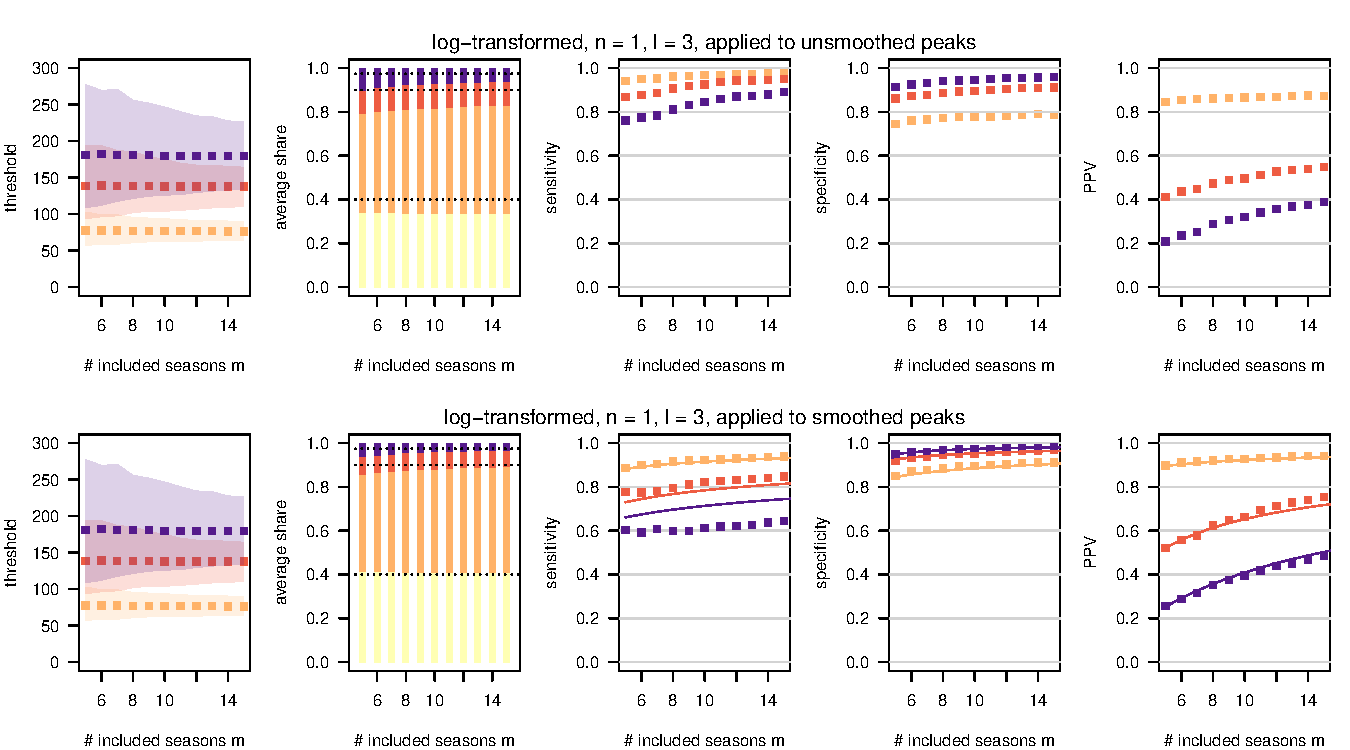
\includegraphics[width=1\textwidth]{figure/plot_smoothing3_us_small.pdf}
\vspace{-33mm}

\caption{Reproduction of Figure \ref{fig:results_smoothing} using US data. Impact of smoothing of historical data on thresholds. We applied a moving average with $l = 3$ to the historical time series prior to computing thresholds and subsequently applied them to either unsmoothed or smoothed new peak values. Results are shown for thresholds computed with a log transformation. See the caption of Figure \ref{fig:results1} for details on the plot elements.}
\label{fig:results_smoothing_us}
\end{figure}


\begin{figure}
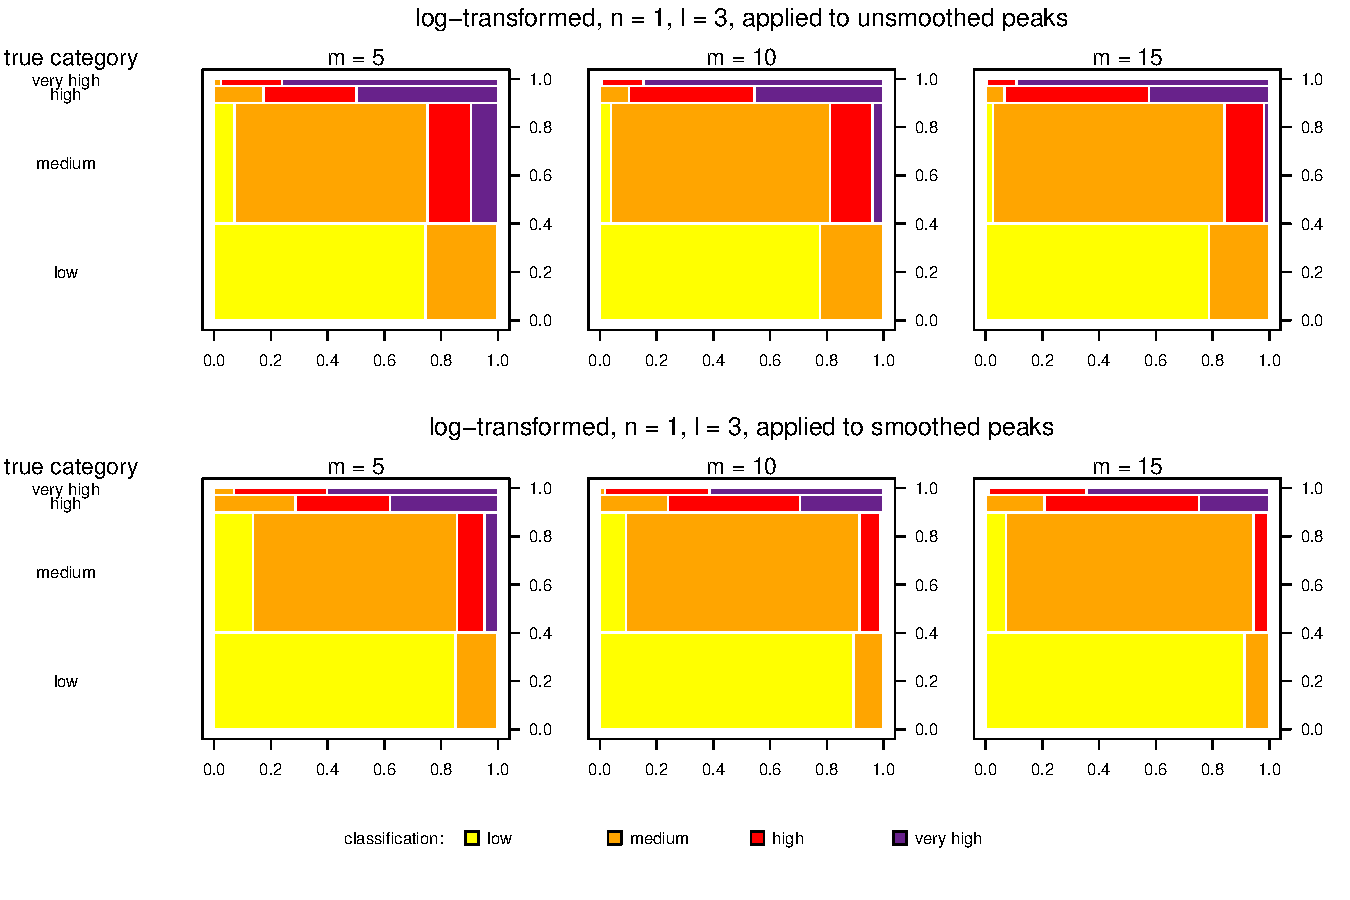
\includegraphics[width=0.95\textwidth]{figure/mosaic_log_smoothed_us.pdf}
\caption{Reproduction of Figure \ref{fig:mosaic_smoothing} using US data. Confusion matrices for intensity classifications obtained with a smoothing window of width $l = 3$ and a log transformation. Top: thresholds applied to unsmoothed new peaks; bottom: thresholds applied to smoothed new peaks. Mosaic plots show which fractions of season peaks which are truly very high, high, medium or low are classified into the four categories, see camption of Figure \ref{fig:mosaic} for details.}
\label{fig:mosaic_smoothing_us}
\end{figure}


\begin{figure}
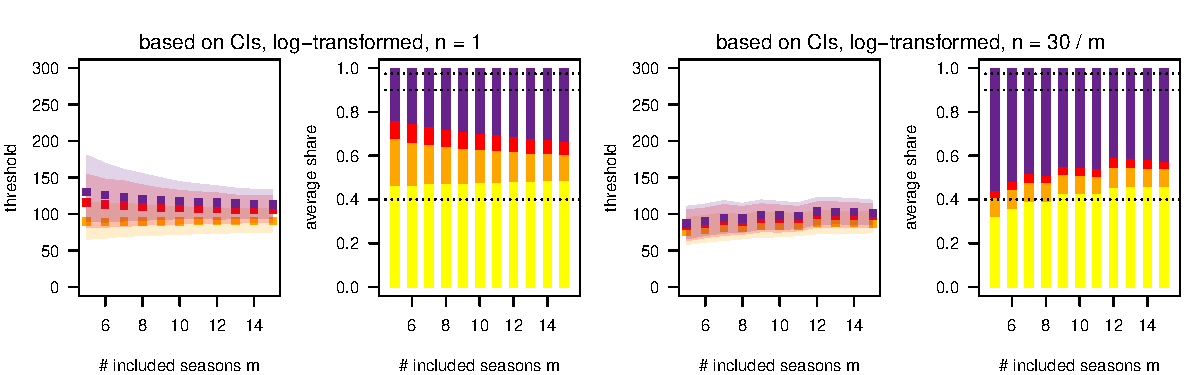
\includegraphics[width=0.93\textwidth]{figure/plot_ci_us.pdf}
\caption{Reproduction of Figure \ref{fig:cis} using US data. Average thresholds and exceedance shares when thresholds are based on confidence intervals rather than prediction intervals. See the caption and legend of Figure \ref{fig:results1} for details on the plot elements.}
\label{fig:cis_us}
\end{figure}

\end{document}